\documentclass[12pt,twoside,a4paper]{book}
\usepackage[pdftex]{graphicx}
\usepackage[pdftex]{hyperref}
\usepackage{epsfig}
\usepackage{a4}
\usepackage[margin=2cm]{geometry}
\pagestyle{headings}

\usepackage{afterpage}
\usepackage{latexsym}
\usepackage{ulem}
\usepackage{natbib}

% macros

\def \ba{\begin{array}}
\def \ea{\end{array}}

\def \be{\begin{equation}}
\def \ee{\end{equation}}

\def \bd{\begin{displaymath}}
\def \ed{\end{displaymath}}

\def \bfl{\begin{flushleft}}
\def \efl{\end{flushleft}}

\def \beqa{\begin{eqnarray}}
\def \eeqa{\end{eqnarray}}

\def \di{\displaystyle}

\def \degrees{^\circ}

\newcommand{\pd}[2]{\frac{\partial #1}{\partial #2}}
\newcommand{\module}{\sf}
\newcommand{\sub}{\it}
\newcommand{\nam}{\it}
\newcommand{\file}{\bf}
\newcommand{\modir}{puma}

% end of macro definition

%------- [PUMA - constants]-------%
\def \dtep{$(\Delta T_R)_{\�P}\;$}
\def \dtepE{$(\Delta T_R)_{EP}\;$}
\def \dtns{$(\Delta T_R)_{NS}\;$}
\def \dtepk{$(\Delta T_R)_{\�P}$}
\def \dtepkE{$(\Delta T_R)_{EP}$}
\def \dtnsk{$(\Delta T_R)_{NS}$}
%---------------------------------%


\begin{document}

\begin{titlepage}
\begin{center}
\begin{figure}
\hspace{1cm}
\parbox{7cm}{

\includegraphics[width=7cm]{Pics/UHH_Logo_RGB}}
\hspace{0.5cm}
\parbox{7cm}{

\includegraphics[width=7cm]{Pics/KC-Logo_RGB}}
\end{figure}

\vspace*{1cm}
{\Huge\bf PUMA} \\
\vspace*{1cm}
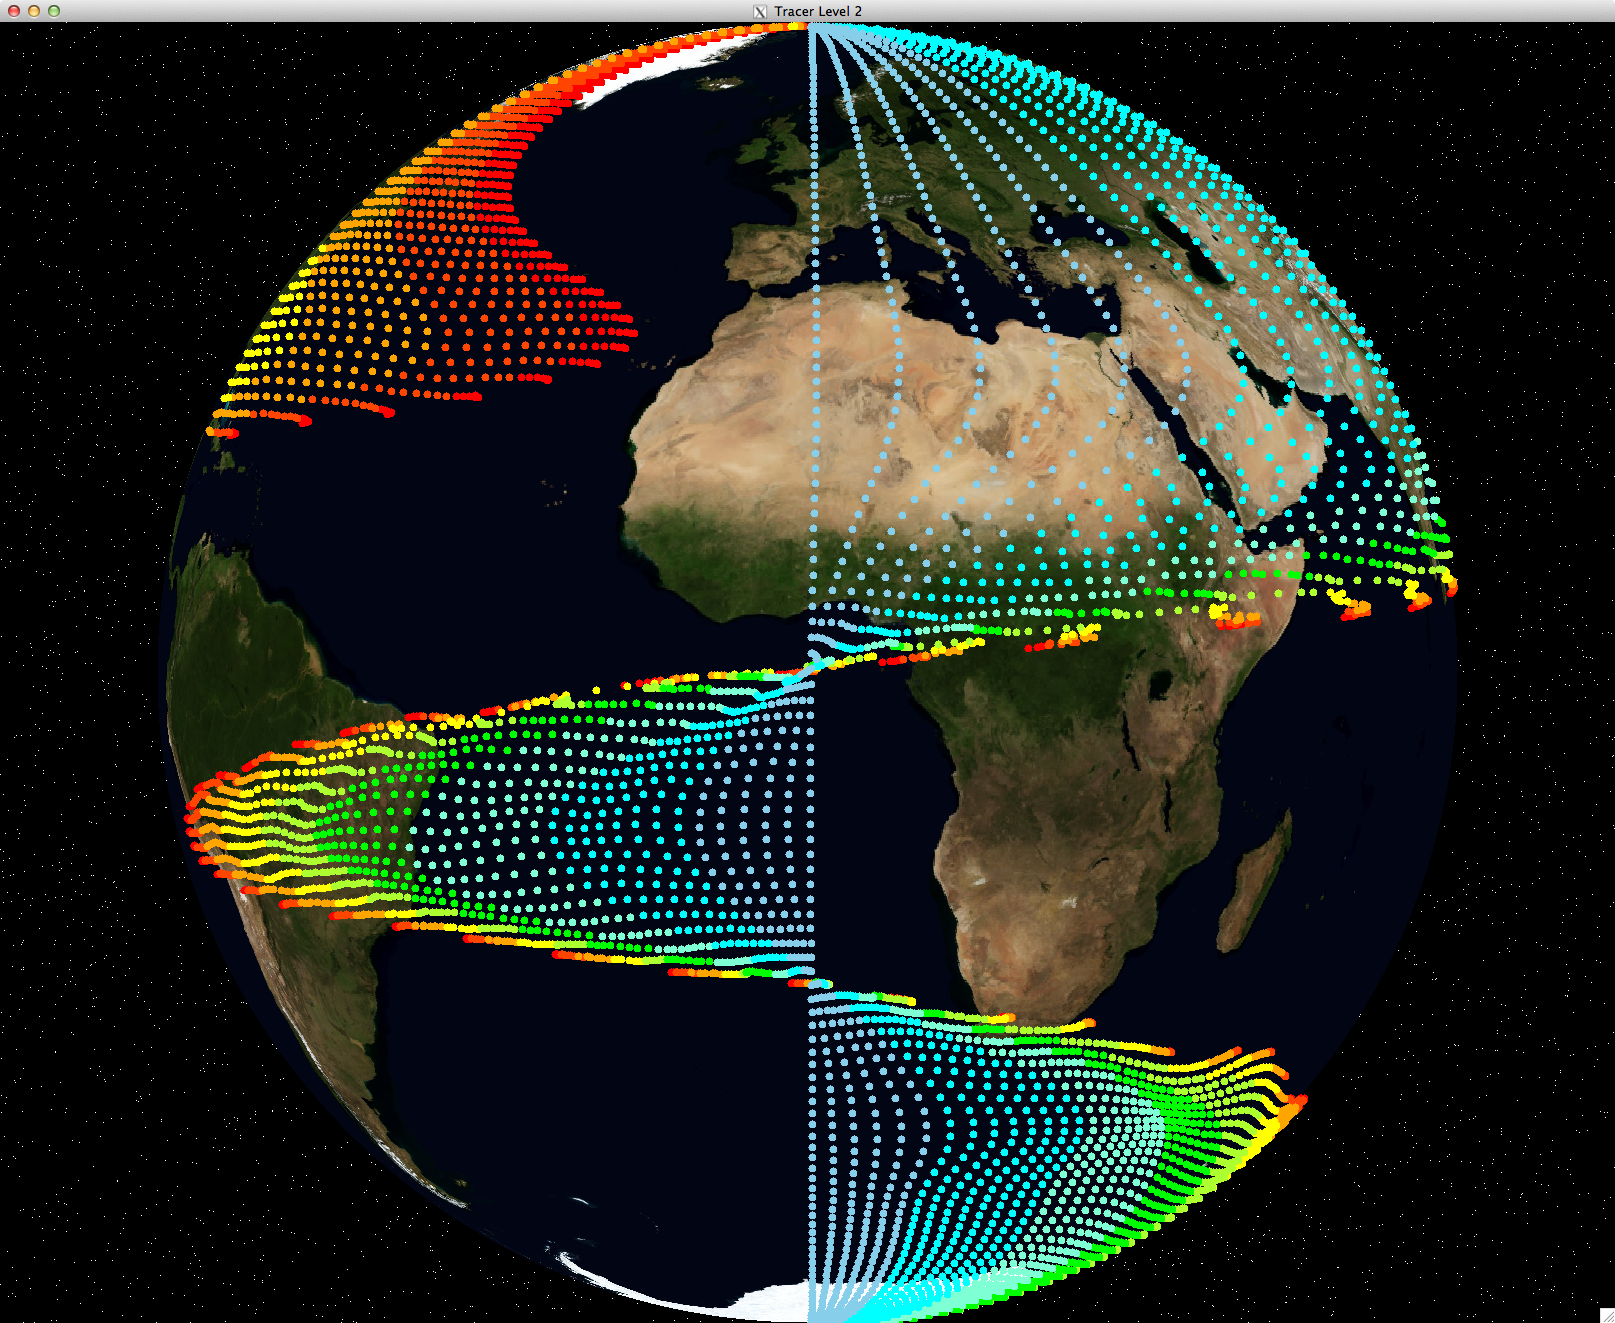
\includegraphics[width=15cm]{Pics/guisnap} \\
\vspace*{1cm}
{\huge \bf User's Guide} \\
\vspace*{1cm}
{\huge \bf Version 17}
\vspace*{1cm}

 Frank Lunkeit -
 Edilbert Kirk       \\
 Klaus Fraedrich -
 Valerio Lucarini    \\
 Simon Blessing -
 Hartmut Borth       \\
 Torben Kunz -
 Alastair McDonald   \\
 Silke Schubert -
 Frank Sielmann      \\

\end{center}
\end{titlepage}

\begin{verbatim}
The PUMA User's Guide is a publication of the
Theoretical Meteorology at the Meteorological Institute of
the University of Hamburg.

Address:

Prof. Dr. Valerio Lucarini
Meteorological Institute
KlimaCampus
University of Hamburg
Grindelberg 5
D-20144 Hamburg
Germany

Contact:

Valerio.Lucarini@uni-hamburg.de.
Frank.Lunkeit@uni-hamburg.de
Edilbert.Kirk@uni-hamburg.de
\end{verbatim}


\bibliographystyle{plainnat}


\tableofcontents

\chapter{Installation}
The whole package containing the models "Planet Simulator" and "PUMA"
along with "MoSt", the "Model Starter" comes in a single file,
usually named "Most(n).tgz" with (n) specifying a version number.
The following subsection gives an example, assuming version 16.

\section{Quick Installation}

\begin{verbatim}
tar -zxvf Most16.tgz
cd Most16
./configure.sh
./most.x
\end{verbatim}

if your tar-command doesn't support the "-z" option (e.g. on Sun UNIX)
type instead:

\begin{verbatim}
gunzip Most16.tgz
tar -xvf Most16.tar
cd Most16
./configure.sh
./most.x
\end{verbatim}

If this sequence of commands produces error messages,
consult the "FAQ" (Frequent Asked Questions) and README files
in the {\most} directory. They are plain text files,
that can be read with the command "more" or any text editor.

\section{{\most}  directory }

\begin{verbatim}
home/Most16> ls -lG

-rw-r--r-- 1   1548 cc_check.c          <- Used by configure.sh
-rwxr-xr-x 1     57 cleanplasim         <- Delete run, bld and bin for PLASIM
-rwxr-xr-x 1     51 cleanpuma           <- Delete run, bld and bin for PUMA
drwxr-xr-x 2   4096 common              <- Topography files
-rwxr-xr-x 1   3911 configure.sh        <- The configure script
-rw-r--r-- 1    308 csub.c              <- Currently unused
-rw-r--r-- 1    234 f90check.f90        <- Used by configure.sh
-rw-r--r-- 1   3033 FAQ                 <- Frequently Asked Questions
drwxr-xr-x 2   4096 images              <- Directory for images
-rw-r--r-- 1    154 makecheck           <- Used by configure.sh
-rw-r--r-- 1     85 makefile            <- Used to "make" most.x
-rw-r--r-- 1 107844 most.c              <- Source for MoSt (Model Starter)
-rw-r--r-- 1   6399 NEW_IN_VERSION_16   <- New in this version
drwxr-xr-x 8   4096 plasim              <- Planet Simulator directory
drwxr-xr-x 2   4096 postprocessor       <- Postprocessor directory
drwxr-xr-x 8   4096 puma                <- PUMA directory
-rw-r--r-- 1    839 README              <- Read this first
-rw-r--r-- 1    191 README_MAC_USER     <- Notes for MAC user
-rw-r--r-- 1    698 README_WINDOWS_USER <- Notes for Windows user
\end{verbatim}

The directory structure must not be changed, even empty directories must be
kept as they are, the Most program relies on the existence of these directories!

For each model, currently "Planet Simulator" and "PUMA" exists a directory
(plasim) and (puma) with following subdirectories:

\begin{verbatim}
Most16/plasim> ls -lg

drwxr-xr-x  2   128  bin   <- model executables
drwxr-xr-x  2  1824  bld   <- build directory
drwxr-xr-x  2   280  dat   <- initial and boundary data
drwxr-xr-x  2    80  doc   <- documentation, user's guide, reference manual
drwxr-xr-x  2   928  run   <- run directory
drwxr-xr-x  2  1744  src   <- source code
\end{verbatim}

After installation only "dat", "doc" and "src" contain files,
all other directories are empty.

Running "Most" to setup a model configuration and define an experiment uses the
directories in the following manner:

\section{Model build phase}

Most writes an executable shell script to the "bld" directory
and executes it directly hereafter.
It copies all necessary source files from "src" to "bld" and modifies
them according to the selected parameter configuration.
Modification of source code is necessary for vertical and horizontal
resolution change and for using more than 1 processor (parallel program
execution). The original files in the "src" directory are not changed by Most.
The program modules are then compiled and linked using the "make" command 
(in bld/most\_plasim\_build),
also issued by Most. Most provides a makefile named make\_\modir \ for
building the executable. For modules that exist in more than one
version the selection of the module to use is done by environment
variables that are set automatically by MoSt but may be changed
manually by the user. Look into the make\_\modir \ for further information.
The resolution and CPU parameters are coded into the filename of the
executable, in order to have different names for different versions.
E.g. the executable "most\_\modir\_t21\_l10\_p2.x" 
is an executable compiled for a horizontal resolution of T21, 
a vertical resolution of 10 levels and 2 CPU's.
The executable is copied to the models "bin" directory after building.
Each time Most is used to setup a new experiment it checks the "bin"
directory for a matching executable. If it's there, it's used without
rebuilding otherwise a new executable with the selected parameters
is created. Rebuilding may be forced by using the clean\modir \ command
in the Most directory.
The build directory is not cleared after usage. The user may want
to modify the makefile or the build script for his own purposes
and start the building directly by executing "most\_\modir\_build".
For permanent user modifications
the contents of the "bld" directories have to be copied elsewhere,
because each usage of Most overwrites the contents of "bld".

\section{Model run phase}

After building the model with the selected configuration,
Most writes or copies all necessary files to the model's
"run" directory. These are the executable, initial and boundary data,
namelist files containing the parameter and finally the
run script itself. Depending on the exit from Most,
either "Save  \& Exit" or "Run \& Exit", the run script is started
from Most and takes control of the model run. A checkmark on
GUI invokes also the 
Graphical User Interface for user control and display
of variables during the run.
Again all contents of the "run" directory are subject of change
for the user. But it would be wise to keep changed run setups
in other, user created directories, because each usage of
Most overwrites the contents of the run directory.

\section{Running long simulations}

For long simulations make a new directory on a filesystem,
that has enough free disk space to store the results.
You may use the "df" command to check filesystems.

Hint 1: Don't use your home directory if there are filequotas.
Your run may crash due to file quota exceeded.

Hint 2: Use a local disk, not NFS mounted filesystems if possible.
The model runs much faster writing output to local disks.

Example:

\begin{itemize}
\item cd {\most}
\item ./most.x
\item Select model and resolution
\item Switch GUI off
\item Switch Output on
\item Edit number of years to run
\item Click on "Save \& Exit"
\item Make a directory, e.g. mkdir /data/longsim
\item cp \modir/run/* /data/longsim
\item cd /data/longsim
\item edit most\_\modir\_run for experiment name
\item edit namelist files if necessary
\item start simulation with most\_\modir\_run \&
\end{itemize}



\chapter{Introduction}
     The {\bf P}ortable {\bf U}niversity {\bf M}odel of the
     {\bf A}tmosphere {\bf (PUMA)} is based on the multi-level spectral
     model {\bf SGCM} ({\bf S}imple {\bf G}lobal {\bf C}irculation
     {\bf M}odel) described by \citep{hossim75} and \citep{jamesgray86}.
     Originally developed as a numerical prediction model,
     it was changed to perform as a circulation model. For example,
     \citep{jamesgray86} studied the influence of surface friction
     on the circulation of a baroclinic atmosphere, \citep{jamesjames92}
      and \citep{JamFraeJam94} investigated ultra-low-frequency
     variability, and \citep{molejames90} analyzed the baroclinic
     adjustment in the context of a zonally varying flow. \citep{frisius98}
      simulated an idealized storm track by embedding
     a dipole structure in a zonally symmetric forcing field and \citep{lunkeit98}
     investigated the sensitivity of GCM scenarios by using
     an adaption technique applicable to SGCMs.
     Storm track dynamics and low frequency variability
     was investigated by \citep{fraedrich2005}. For further citations search the
     bibliography at the end of this document and the list of publications at 
     {\url{http://www.mi.uni-hamburg.de/puma}}.

    
     PUMA was created with following aims in mind: training of junior
     scientists, compatibility with the {\bf ECHAM} 
     ({\bf E}uropean {\bf C}entre - {\bf HAM}burg) model and as a tool for
     further scientific investigations.
     

\section{Training of junior scientists and students}
     PUMA contains only the main processes necessary to simulate
     the atmosphere. The source code is short and clearly arranged.
     A student can learn to work with PUMA within a few weeks, whereas a
     full size GCM requires a team of specialists for maintenance,
     experiment design and diagnostics.
    
\section{Compatibility with other models}
     PUMA is designed to be compatible with other
     circulation models like Planet Simulator and ECHAM.
     The same triangular truncation is employed,
     and analogous transformation techniques like the Legendre- and
     Fast-Fourier transformation are used.
     The postprocessor {\bf Pumaburner} differs from ECHAM's
     {\bf Afterburner} only in respect to the format of the model's
     raw data which overcomes some problems of the ECHAM data format.
     PUMA uses a more compact though more precise
     format compared to the {\bf GRIB} ({\bf GRI}dded {\bf B}inary),
     which is used for ECHAM output.
     The Pumaburner supports the output formats SERVICE and
     NetCDF. All diagnostics and graphics software that are used with the
     ECHAM/Afterburner data can be used with PUMA/Pumaburner
     in exactly the same way.

\pagebreak
    
\begin{figure}
\centering
\begin{minipage}{0.75\linewidth}
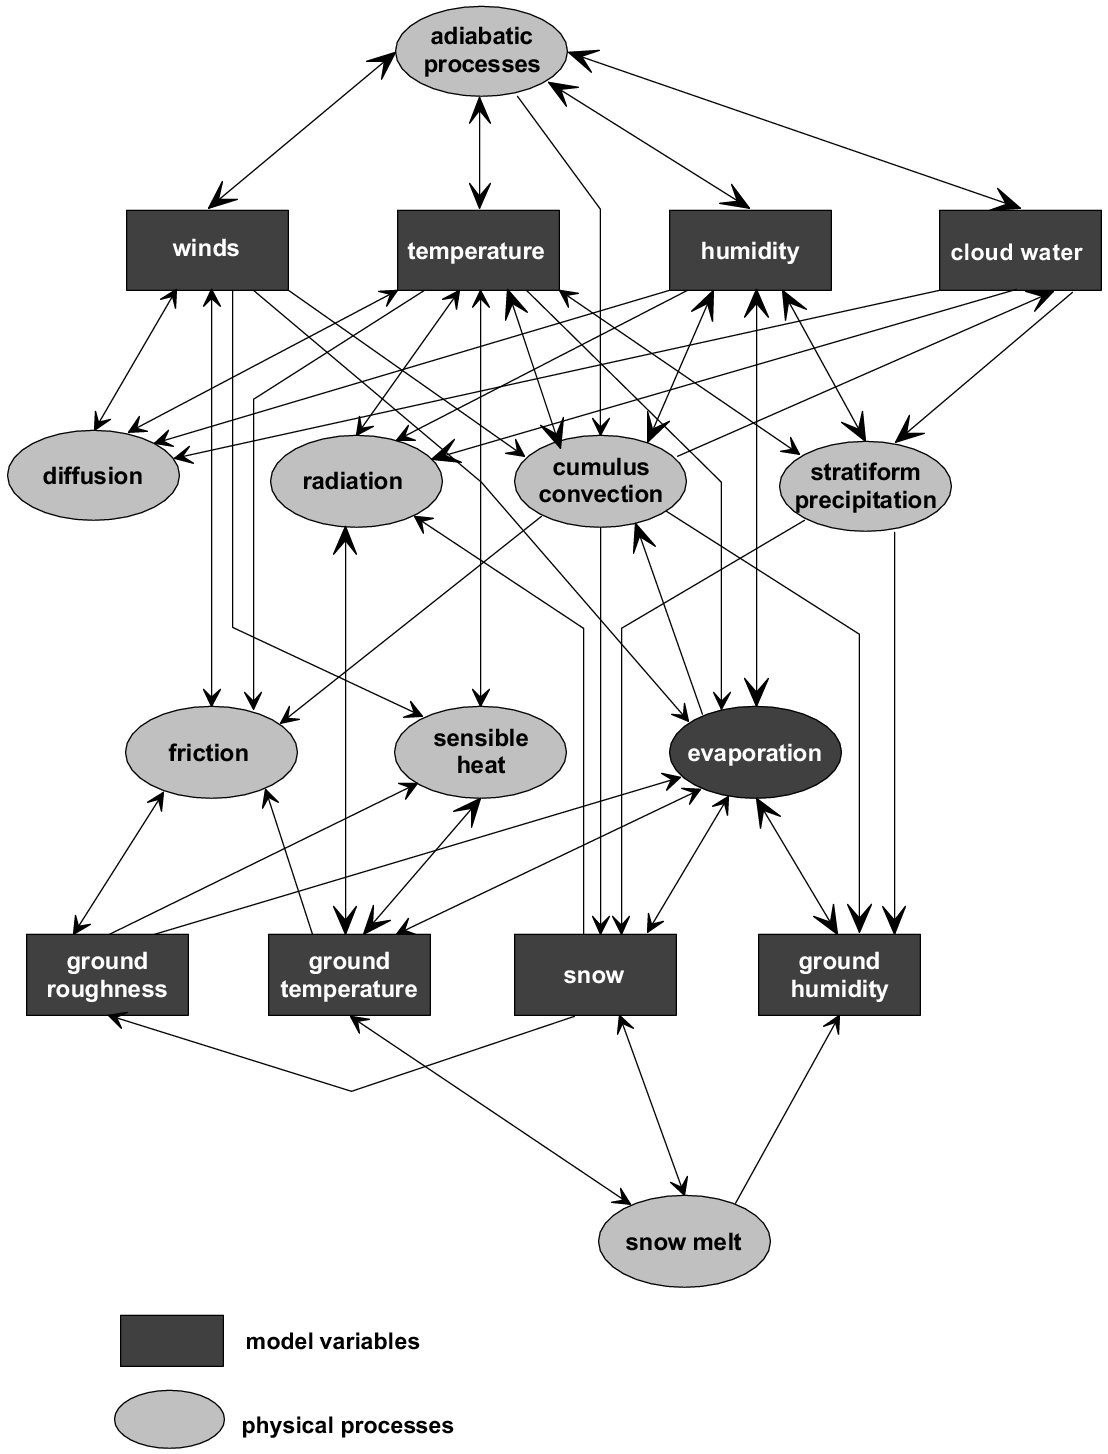
\includegraphics[height=15cm]{Pics/Processes_ECHAM}
%\centering \epsfig{figure=Tr_z.Eng.eps, width=\linewidth}
\end{minipage}
\setlength{\unitlength}{1cm}

\vspace{-2cm}

\begin{minipage}{.5\linewidth}
\begin{picture}(6,8)
\thicklines

\newsavebox{\ovalbox}
\savebox{\ovalbox}(0,0){
   \thicklines
   \put(0,-0.5){\oval(2.0,0.7)}}
\newsavebox{\frbox}
\savebox{\frbox}(0,0){
   \thicklines
   \put(0,-0.5){\framebox(2.0,0.7)}}

\put(4,4.2){\usebox{\ovalbox}}
\put(3.35,3.95){\scriptsize \shortstack[c]{Adiabatic \\ processes}}

\put(4,3.75){\vector(3,-2){1.5}}
\put(5.5,2.75){\vector(-3,2){1.5}}
\put(4,3.75){\vector(-3,-2){1.5}}
\put(2.5,2.75){\vector(3,2){1.5}}

\put(1.5,2.4){\usebox{\frbox}\makebox(2.05,0){\scriptsize Winds}}
\put(4.5,2.4){\usebox{\frbox}\makebox(2.1,0){\scriptsize Temperature}}

\put(2.5,2.05){\vector(0,-1){1.05}}
\put(2.5,1.05){\vector(0,1){1.}}
\put(5.5,2.05){\vector(0,-1){1.05}}
\put(5.5,1.05){\vector(0,1){1.}}

\put(2.5,0.7){\usebox{\ovalbox}}
\put(2.5,0.6){\makebox(0,0){\scriptsize Friction}}
\put(5.5,0.7){\usebox{\ovalbox}}
\put(4.95,0.4){\scriptsize \shortstack[c]{Diabatic \\ heating}}

\end{picture}
\end{minipage}

\vspace{1cm}

\caption{Processes in ECHAM (a) and PUMA (b)}
\label{ProcessesFig}
\end{figure}

\section{Scientific applications}
     The PUMA code is the dynamical core of a GCM forced by Newtonian
     cooling and Rayleigh friction, such as that proposed by Held \&
     Suarez (1994) to evaluate the dynamical cores of GCMs. It forms
     the basis for various applications:
\begin{itemize}
   \item The code can be utilized
     to build and test new numerical algorithms (like semi-Langrangian
     techniques).
   \item Idealized experiments can be performed to analyze nonlinear
     processes arising from internal atmospheric systems (life cycles,
     etc.).
   \item Data assimilation techniques can be incorporated to
     interpret results from GCM simulations or observations.
\end{itemize}

    Figure \ref{ProcessesFig} (a) demonstrates the complexity of the 
    interactions in a full size climate model, which leads to similar 
    complex response patterns from small parameter changes. The same 
    diagram for PUMA Figure \ref{ProcessesFig} (b) shows the simple 
    and direct paths which allow the easy identification of the effects 
    from changes to this model.

\section{Requirements}
   PUMA is open source, everyone may download and use it.
   Though it's easy to use,
   the design of experiments and the interpretation of the results
   require a thorough knowledge of atmospheric science.

   PUMA is available as FORTRAN-90 source code. So all that is needed
   to use PUMA on any computer is a FORTRAN-90 compiler.
   The GUI additionally requires a C-compiler with the graphical
   library X11, which is standard on any UNIX/Linux system
   as well as on newer MACs.
   Windows user may try a X11-emulator like Cygwin.

   The program was developed and tested with several operating systems
   including LINUX, MAC-OS, and Solaris. The main development was done
   using Linux and MAC-OS and the FORTRAN compiler gfortran and sunf90.

   The postprocessor Pumaburner requires a C++ compiler.

   There are several compilers available for the Linux operating system.
   MoSt, PUMA, and Planet Simulator were successfully tested with:

\begin{itemize}
\item SunStudio12 (development environment including
   FORTRAN-90, C, C++, and Debugger) for Solaris and Linux.
   SunStudio12 can be downloaded for free from {\url{http://www.sun.com}}.
\item Gnu FORTRAN (gfortran).
   This free and open access FORTRAN-90 compiler is part of most
   Linux distributions.
   It's also available from
   {\url{http://directory.fsf.org/devel/compilers/gfortran.html}}.
\end{itemize}




\section{History}
    
    The University of Hamburg PUMA model originates from
     the Hoskins \& Simmons SGCM ({\bf S}imple {\bf G}eneral {\bf C}irculation {\bf M}odel)
     version (\citep{hossim75}). The major differences between PUMA
     and its predecessor SGCM are:

\begin{itemize}
   \item The code is rewritten in portable
     FORTRAN-90 code, which removes problems associated with
     machine-specific properties like word lengths, floating point
     precision, output, etc. All the necessary routines are
     in the source code including the
     FFT ({\bf F}ast {\bf F}ourier {\bf T}ransformation)
     and the Legendre Transformation. The model can be run
     on any computer with a standard FORTRAN-90 compiler.
     The MPI-library is needed to run
     PUMA on parallel machines (see below).
     The Xlib (X11R6) library is needed for the graphical user
     interface.
   \item  The
     truncation scheme is changed from the jagged triangular truncation
     to the standard triangular truncation scheme making it compatible to other
     T-models like ECHAM.

   \item  The PUMA/Pumaburner system is data compatible to ECHAM/Afterburner.
     Thus all other ECHAM diagnostic software can be used on PUMA data.

   \item PUMA is fully parallelized and can use as many CPU's 
    as half of the number of latitudes (e.g. 16 in T21 resolution). It uses the MPI
    ({\bf M}essage {\bf P}assing {\bf I}nterface) library while
    running on parallel systems or a cluster.
    MPI is not needed for running PUMA on a single CPU.

   \item  The ongoing development added several new features like the preprocessor,
   graphical user interface, spherical harmonics mode selection, and many more.

\end{itemize}


\nocite{KunzFraeLun09}
\nocite{Perez2005}
\nocite{Blessetal2008}
\nocite{fraelun2008}
\nocite{KunzFraeKirk2008}

\chapter{Horizontal Grid}

\begin{figure}
   \centering
   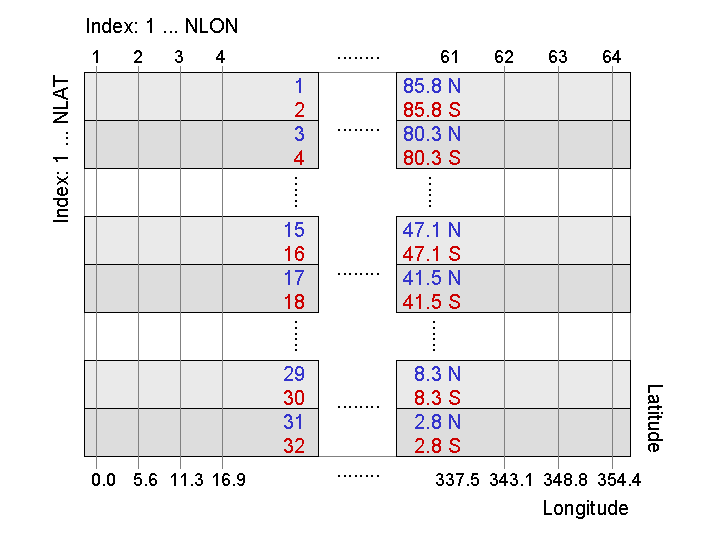
\includegraphics[width=14cm]{Pics/PUMA_alternate_grid.png}
   \caption[]{PUMA T21 horizontal grid sorted by index}
   \label{pumat21igrid}
\end{figure}

PUMA uses internally (other than the Planet Simulator and PUMA version 15) an alternating Gaussian grid.
This feature is unimportant for users, who don't change source code - the output file
will still contain the usual Gaussian grid with the latitude index running from the most Northern latitude
to the most Southern one. But for those, who fiddle around with the code or want to implement additional
arrays it is important to understand the internal structure.

The alternating grid was introduced for two reasons:

1) The number of values for Legendre polynomials could be reduced by a factor of two, because 
pairs of Northern and Southern latitudes with the same absolute value can be processed
simultaneously. This is especially useful for very high resolution runs.
E.g. a PUMA T1365 needs now ca. 45 GByte memory.

2) The Legendre transformation was recoded to use symmetric and antisymmetric Fourier
coefficients for these latitude pairs resulting in strict conservation of symmetry
and antisymmetry properties.

Figure \ref{pumat21igrid} shows how the elements of a horizontal grid
are stored in computer memory. The restrictions for parallel execution
using alternating grids are:

Because a latitude pair must not be separated to different processes,
the maximum number of processes is half of the number of latitudes.
Also it not possible to use an odd number of processes.


Figure \ref{pumat21lgrid} shows a horizontal grid sorted from North to South
and its corresponding latitude indices.

The subroutines ALT2REG and REG2ALT (in legsym.f90) may be used to convert from
alternating to regular Gaussian grid and vice versa.




\begin{figure}
   \centering
   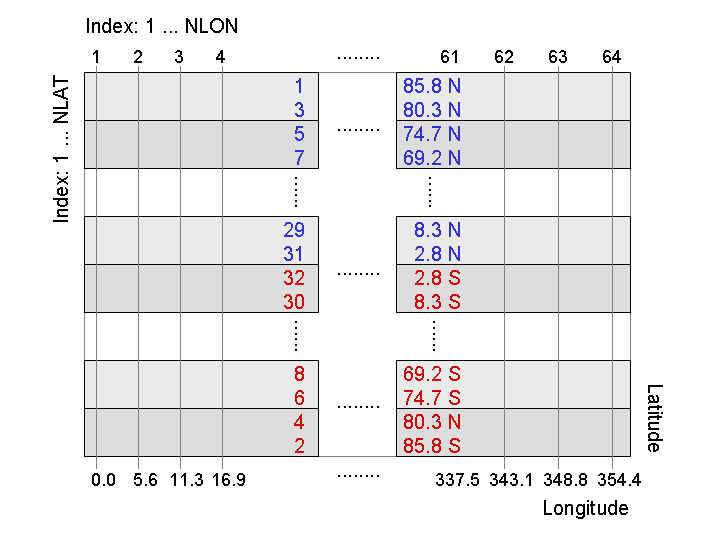
\includegraphics[width=14cm]{Pics/PUMA_alternate_grid_geogr.png}
   \caption[]{PUMA T21 horizontal grid sorted from North to South}
   \label{pumat21lgrid}
\end{figure}



\chapter{Modules}
This is the technical documentation of the PUMA model. In the following, the purpose of each
module is given and its general structure and possible input and output
parameters provided (namelist, files) are explained. 

%--------------------------------------------------------------------------------

\begin{center}
\begin{tabular}{|p{15cm}|}
\hline
\vspace{-5mm} \section{fftmod.f90 / fft991mod.f90} \vspace{-5mm} \\
\hline
\vspace{1mm} {\bf General} The module {\module fftmod.f90} contains all subroutines
necessary to perform the fast fourier transformation and its inverse. The interface to the main
PUMA module {\module puma.f90}
is given by the subroutines {\sub gp2fc} and {\sub
fc2gp} which are called in {\module puma.f90} from the subroutine {\sub gridpoint}.  \vspace{3mm} \\
\hline
\vspace{1mm} {\bf Input/Output} {\module fftmod.f90} does not use any additional input or
output files. No namelist input is required. \vspace{3mm} \\
\hline
\vspace{2mm} {\bf Structure} Internally, {\module fftmod.f90} uses the FORTRAN-90 module
{\module fftmod}, which uses no other modules. Subroutine {\sub gp2fc} performs the
transformation from gridpoint space into fourier space while the subroutine {\sub fc2gp} does
the transformation from fourier space into grid point space. Both routines use several
subroutines
to do the direct or indirect transformation for different factors. When {\sub gp2fc} or {\sub
fc2gp} is called for the first time, {\sub fftini} is called to initialize the FFT.
\vspace{3mm} \\
\hline
\vspace{2mm} Alternatively, the module {\module fft991mod.f90} may be used
instead of {\module fftmod.f90}. While {\module fftmod.f90} runs faster,
{\module fft991mod.f90} can be used for resolutions that are not supported by {\module fftmod.f90}, e.g. T63 or T106.
To select the appropriate module edit the file "Most15/puma/src/make\_puma".
Use either:
\begin{verbatim}
FFTMOD=fftmod
\end{verbatim}
or
\begin{verbatim}
FFTMOD=fft991mod
\end{verbatim}
\vspace{3mm} \\
\hline
\end{tabular}
\end{center}
\newpage

%---------------------------------------------------------------------------------------------

\begin{center}
\begin{tabular}{|p{15cm}|}
\hline
\vspace{-5mm} \section{guimod.f90 / guimod\_stub.f90} \vspace{-5mm} \\
\hline
\vspace{1mm} {\bf General} The module {\module guimod.f90}
contains subroutines for communication with the GUI.
On operating systems that do not support the Xlib library (X11R6) e.g. Windows,
{\module guimod\_stub.f90} may be used as a stub replacement.
\vspace{3mm} \\
\hline
\vspace{2mm} {\bf Structure}
The following subroutines are included in {\module guimod.f90}:

\begin{center}
\begin{tabular}{l p{2cm} l}
Subroutine & &Purpose \\
&& \\
{\sub guistart} && initialize the GUI \\
{\sub guistop}  && finalize the GUI \\
{\sub guistep\_puma} && called every timestep from PUMA \\
{\sub guistep\_plasim} && called every timestep from PLASIM \\
{\sub guips} && gather, scale, and send surface pressure to the GUI \\
{\sub guihor} && gather, scale, and send a gridpoint array to the GUI \\
{\sub guigv} && gather, scale, and send wind components to the GUI \\
{\sub change\_disp} && called for user input into the GUI \\
{\sub change\_dtep} && called for user input into the GUI \\
{\sub change\_dtns} && called for user input into the GUI \\
{\sub change\_co2} && called for user input into the GUI \\
{\sub change\_gsol0} && called for user input into the GUI \\
{\sub change\_dawn} && called for user input into the GUI \\
\end{tabular}
\end{center}
\vspace{3mm} \\
\hline
\end{tabular}
\end{center}
\newpage

%---------------------------------------------------------------------------------------------

\begin{center}
\begin{tabular}{|p{14cm}|}
\hline
\vspace{-5mm} \section{legsym.f90} \vspace{-5mm} \\
\hline
\vspace{1mm} {\bf General} The module {\module legsym.f90}
 contains all the subroutines
necessary to perform the Legendre transformation and its inverse.
The module legsym is written for arrays in alternate representation,
which use pairs of Northern and Southern latitudes. This symmetry conserving
scheme is different to the Legendre modules used in PLASIM or the preprocessor.

 The interface to the main
PUMA module {\module puma.f90} is given by the subroutines {\sub legini}, {\sub
inigau}, {\sub fc2sp}, {\sub fc3sp}, and {\sub sp2gp}
 which are called in {\module puma.f90}
from the subroutines {\sub prolog} and {\sub gridpoint}.
\vspace{3mm} \\
\hline
\vspace{1mm} {\bf Input/Output} {\module legsym.f90}
 does not use any other input or output files. No namelist input is required. 
 \vspace{3mm} \\
\hline
\vspace{1mm}
The following subroutines are included in {\module legsym.f90}:

\begin{center}
\begin{tabular}{l p{2cm} l}
Subroutine & &Purpose \\
&& \\
{\sub inigau} && compute Gaussian abscissae and weights \\
{\sub legini} && compute Legendre polynomials \\
{\sub fc2sp}  && Fourier to Spectral transformation \\
{\sub fc2spdmu}  && Fourier to Spectral transformation with d/dmu \\
{\sub sp2fc}  && Spectral to Fourier transformation \\
{\sub sp3fc}  && simultaneous transformation of T, Div., and Vort. \\
{\sub mktend} && compute and transform tendencies \\
{\sub reg2alt} && convert regular array to alternate array \\
{\sub alt2reg} && convert alternate array to regular array \\
\end{tabular}
\end{center}
\vspace{3mm} \\
\hline
\end{tabular}
\end{center}
\newpage

%--------------------------------------------------------------------------------
\begin{center}
\begin{tabular}{|p{15cm}|}
\hline
\vspace{-5mm} \section{mpimod.f90 / mpimod\_stub.f90} \vspace{-5mm}
\\
\hline
\vspace{1mm} {\bf General} The module {\module mpimod.f90} contains the interface
subroutines of the MPI ({\bf M}essage {\bf P}assing {\bf I}nterface) needed for 
(massive) parallel computing.  Several MPI
routines are called from the module. The interface to the other modules is provided by numerous
subroutines with names which begin with {\sub mp}. Subroutines in {\module mpimod.f90}  are
called from several other modules. There  are no direct calls to the MPI other than
from within {\module mpimod.f90}. This encapsulation makes it possible to
use {\module mpimod\_stub.f90} for single CPU runs without
changing any other part of the model code.
The selection is done automatically when using MoSt, or can be done manually
by editing "Most16/puma/src/make\_puma".  \vspace{3mm} 
\\
\hline
\vspace{1mm} {\bf Input/Output} {\module mpimod.f90} and {\module mpimod\underline{
}stub} do not use any extra input or
output files. No namelist input is required. \vspace{3mm} \\
\hline
\vspace{2mm} {\bf Structure} Internally, {\module mpimod.f90} uses the FORTRAN-90
module
{\module mpimod},  which in turn uses the global common module {\module pumamod} from
{\module pumamod.f90} and the MPI module {\module mpi}. {\module mpimod\underline{
}stub.f90} does not use any other module. The following subroutines are included in {\module
mpimod.f90}:

\begin{center}
\begin{tabular}{l p{2cm} l}
Subroutine & &Purpose \\
&& \\
{\sub mpbci} && broadcast 1 integer \\
{\sub mpbcin} & &broadcast n integers \\
{\sub mpbcr} & &broadcast 1 real \\
{\sub mpbcrn} & &broadcast n reals \\
{\sub mpbcl} && broadcast 1 logical \\
{\sub mpscin} & &scatter n integers \\
{\sub mpscrn} && scatter n reals \\
{\sub mpscgp} && scatter grid point field \\
{\sub mpgagp} && gather grid point field \\
{\sub mpgallgp} && gather grid point field to all \\
{\sub mpscsp} & &scatter spectral field \\
{\sub mpgasp} && gather spectral field \\
{\sub mpgacs} && gather cross section \\
{\sub mpgallsp} && gather spectral field to all \\
{\sub mpsum} && sum spectral field \\
{\sub mpsumsc} && sum and scatter spectral field \\
{\sub mpsumr} && sum n reals \\
{\sub mpsumbcr}& & sum and broadcast n reals \\
{\sub mpstart} & &initialize MPI \\
{\sub mpstop} & &terminate MPI \\
\end{tabular}
\end{center}
\vspace{3mm} \\
\hline
\end{tabular}
\end{center}

\newpage

\begin{center}
\begin{tabular}{|p{15cm}|}
\hline
\begin{center}
\begin{tabular}{l p{2cm} l}
Subroutine & &Purpose \\
&& \\
{\sub mpreadgp}& & read and scatter grid point field \\
{\sub mpwritegp}& & gather and write grid point field \\
{\sub mpwritegph} && gather and write (with header) grid point field \\
{\sub mpreadsp} & &read and scatter spectral field \\
{\sub mpwritesp} &&gather and write spectral field \\
{\sub mpi\_info} && report information about setup \\
{\sub mpgetsp}   && read spectral array from restart file \\
{\sub mpgetgp}   && read gridpoint array from restart file \\
{\sub mpputsp}   && write spectral array to restart file \\
{\sub mpputgp}   && write gridpoint array to restart file \\
{\sub mpmaxval}  && compute maximum value of an array \\
{\sub mpsumval}  && compute sum of all array elements \\
\end{tabular}
\end{center}

\vspace{3mm} \\

\hline
\end{tabular}
\end{center}
\newpage
%--------------------------------------------------------------------------------

\begin{center}
\begin{tabular}{|p{15cm}|}
\hline
\vspace{-5mm} \section{puma.f90} \vspace{-5mm} \\
\hline
\vspace{1mm} {\bf General} The module {\module puma.f90}
is the main module of the
model. It includes the main program {\sub puma} and controls the run.
The interface routines to all other modules are
called from {\module puma.f90}.
The output is performed by calling the subroutine to {\module outsp}, and
the adiabatic tendencies and the horizontal
diffusion are also computed in {\module puma.f90}.
To do the necessary transformations, calls to the modules {\module fftmod.f90}
and {\module legsym.f90} are used. \vspace{3mm} \\
\hline
\vspace{1mm} {\bf Input/Output} {\module puma.f90}
A diagnostic printout is written to the standard output
(usually redirected with the operator "$>$" to a file). {\module puma.f90} is
controlled by the namelist {\nam inp} which is part of the namelist file {\file
puma$\_$namelist}. For a complete list of namelist variables see
Appendix C. Here is a table of the most important ones:

\vspace{1mm} 

\begin{center}
\begin{tabular}{l l p{6cm} c}
Parameter & Type & Purpose & Default \\
&&&\\
MPSTEP & Integer & MPSTEP (Minutes Per STEP) defines the length of the
                   time step. Recommended values are 60 min. for T21
                   and 20 min for T42. The values are not checked
                   so take care not to violate the CFL
                   (Courant-Friedrichs-Levy) criterion!  & 60 \\
NYEARS  & Integer & Number of years to be run & 1 \\
NMONTHS & Integer & Number of months to be run : NYEARS and NMONTHS
                    may be used together. The simulation length in
                    days is: NYEARS * 360 + NMONTHS * 30.  & 0 \\
NOUTPUT & Integer & NOUTPUT is a global switch for enabling (1)
                    or disabling (0) writing to {\bf puma\_output}.   & 1 \\
NWPD    & Integer & NWPD (Number of Writes Per Day) defines the
                    output interval for writing model arrays to the
                    file {\bf puma\_output}. Possible values range
                    from 1 (daily output) to 24 (hourly).   & 1 \\
NDIAG   & Integer & NDIAG sets the interval (in time steps) for 
                    printing out some diagnostic arrays and values
                    to the standard output.   & 12 \\
\end{tabular}
\end{center}
\vspace{3mm} \\
\hline
\end{tabular}
\end{center}

\newpage 

\begin{center}
\begin{tabular}{|p{15cm}|}
\hline
\begin{center}
\begin{tabular}{l l p{5cm} c} %{p{3cm} p{2cm} p{6cm} p{2cm}}
Parameter & Type & Purpose & Default \\
&&&\\
NDL(NLEV) & Integer Array & Switch for diagnostic print out of a level (0~=~off; 1~=~on)
& NLEV $\cdot$ 0 \\
DTEP  & Real & Equator to pole temperature difference [K] for Newtonian cooling & 60.0 \\ 
DTNS  & Real & North to South pole temperature difference [K] for Newtonian cooling & 0.0 \\   
DTROP & Real & Tropopause height [m] for Newtonian cooling & 12000.0 \\  
DTTRP & Real & Smoothing of the tropopause [K] for Newtonian cooling & 2 \\
TGR   & Real & Surface temperature [K] for Newtonian cooling & 288 \\
TDISS & Real & Time scale [d] for the horizontal diffusion & 0.25 \\
PSURF & Real & Global mean sea level pressure [Pa] & 101100.00 \\
RESTIM(NLEV)  & Real Array & Time scale [d] for Newtonian cooling & 0.0 \\
T0K(NLEV)  & Real Array & Reference temperature used in the discretization scheme & 250.0 \\
TFRC(NLEV) & Real Array & Time scale [d] for Rayleigh friction (0.0~=~off)& 0.0
\end{tabular} 
\end{center}
\vspace{3mm} \\
\hline

\vspace{2mm} {\bf Structure}
After starting MPI, the main program {\sub puma} calls {\sub
prolog} to initialize the model. Then {\sub master} is called to do the time stepping.
Finally, subroutine {\sub epilog} terminates the run. In subroutine {\sub prolog} calls to
different subroutines, which are part of {\module puma.f90} or are  provided by other
modules, initialize various parts of the model: {\sub gauaw} and {\sub inilat} build  the grid,
{\sub readnl} reads the namelist file and sets parameters using the namelist input,
{\sub initpm} and {\sub initsi} initialize parameters for the physics and the semi
implicit scheme respectively, and {\sub outini} starts the output.
The program then checks for the existence of a file named "puma\_restart".
If the file can be opened then the restart record
is read by {\sub restart}, otherwise {\sub initfd} sets the prognostic variables 
to their initial values.
Finally, the global averaged surface
pressure is set using PSURF and the orography. The subroutine {\sub master} controls the
time stepping. First, if it is not a restart, the initial NKITS explicit forward time steps are
performed.
The main loop is defined by calling {\sub gridpoint} to set the nonlinear tendencies,
and {\sub spectral} to add the linear tendencies. The run is finalized by subroutine
{\sub epilog} which writes the restart records and terminates the MPI. \vspace{3mm} \\
\hline
\end{tabular}
\end{center}
\newpage
 %---------------------------------------------------------------------------------------
\begin{center}
\begin{tabular}{|p{15cm}|}
\hline
\vspace{-5mm} \section{pumamod.f90} \vspace{-5mm} \\
\hline
\vspace{1mm} {\bf General} The module {\module pumamod.f90} contains all the parameters
and
variables which may be used to share information between {\module puma.f90} and other
modules. No subroutines or programs are included. \vspace{3mm} \\
\hline
\vspace{1mm} {\bf Input/Output} {\module pumamod.f90} does not use any extra input
or output files. No namelist input is required. \vspace{3mm} \\
\hline
\vspace{2mm} {\bf Structure} Internally, {\module pumamod.f90} is a FORTRAN-90
module named {\module pumamod}. Names for global parameters, scalars and arrays are
declared and, if possible, values are preset.\vspace{3mm} \\
\hline
\end{tabular}
\end{center}
\newpage

%---------------------------------------------------------------------------------------------
\begin{center}
\begin{tabular}{|p{15cm}|}
\hline
\vspace{-5mm} \section{restartmod.f90} \vspace{-5mm} \\
\hline
\vspace{1mm} {\bf General} The module {\module restartmod.f90}
contains routines for opening, reading and writing the restart files.
The scalars and arrays of the restart files
are identified by name. This enables adding or removing
variables from the restart files without loosing compatibility.
There is also no dependence on the sequence of variables.
In parallel runs 
these routines are either called from the root process,
which takes care of broadcasting, or from subroutines in
{\module mpimod.f90} which gather before writing,
or scatter after reading, the arrays.
\vspace{3mm} \\
\hline
\vspace{2mm} {\bf Structure}
\begin{center}
\begin{tabular}{l p{2cm} l}
Subroutine & &Purpose \\
&& \\
{\sub restart\_ini} && Scan restart file and store pointer \\
{\sub restart\_prepare} && Open file for restart ouput \\
{\sub restart\_stop} && Close files \\
{\sub get\_restart\_integer} && Read integer scalar \\
{\sub get\_restart\_array} && Read real array \\
{\sub put\_restart\_integer} &&  Write integer scalar \\
{\sub put\_restart\_array}   && Write real array \\
{\sub fileseek} && position filepointer to requested variable \\
{\sub check\_equality} && May be used as debug tool \\
\end{tabular}
\end{center}

\vspace{3mm} \\
\hline
\end{tabular}
\end{center}
\newpage

%---------------------------------------------------------------------------------------------


\chapter{Parallel Program Execution}
\section{Concept}

The {\bf Planet Simulator} is coded for parallel execution
on computers with multiple CPU's or networked machines.
The implementation uses MPI (Message Passage Interface),
that is available for nearly every operating system
{\url{http://www.mcs.anl.gov/mpi}}.

In order to avoid maintaining two sets of source code
for the parallel and the single CPU version, all
calls to the MPI routines are encapsulated into a module.
Users, that want to compile and execute the parallel
version use the module
{\bf mpimod.f90} and the commands {\bf mpif90}
for compiling and {\bf mpirun} for running.

If MPI is not implemented or the single CPU
version is sufficient, {\bf mpimod\_stub.f90}
is used instead of {\bf mpimod.f90}.
Also remove or comment the line:
\begin{verbatim}
!     use mpi
\end{verbatim}
and set the number of processors to 1:
\begin{verbatim}
      parameter(NPRO = 1)
\end{verbatim}




\section{Parallelization in Gridpoint Domain}

The data arrays in gridpoint domain are either 
three-dimensional e.g. gt(NLON, NLAT, NLEV) referring
to an array organized after longitudes, latitudes and levels,
or two-dimensional, e.g. gp(NLON, NLAT).
The code is organized such, that there are no dependencies
in latitudinal direction, while in gridpoint domain.
Such dependencies are resolved during the Legendre-Transformations.
So the the partitioning of the data is done in latitudes.
The program can use as many CPU's as latitudes with the extreme
of every CPU doing the computations for a single latitude.
There is the restriction however, that the number of latitudes
(NLAT) divided by the number of processors (NPRO), giving
the number of latitudes per process (NLPP) must have zero
remainder. E.g. A T31 resolution uses $NLAT=48$.
Possible values for NPRO are then 1, 2, 3, 4, 6, 8, 12, 16, 24, and 48.

All loops dealing with a latitudinal index look like:
\begin{verbatim}
      do jlat = 1 , NLPP
         ....
      enddo
\end{verbatim}

There are, however, many subroutines, with the most prominent
called {\bf calcgp}, that can fuse latitudinal and longitudinal
indices. In all these cases the dimension NHOR is used.
NHOR is defined as: $NHOR = NLON * NLPP$ in the 
pumamod - module. The typical gridpoint loop that looks like:

\begin{verbatim}
      do jlat = 1 , NLPP
         do jlon = 1 , NLON
            gp(jlon,jlat) = ...
         enddo
      enddo
\end{verbatim}

is then replaced by the faster executing loop:

\begin{verbatim}
      do jhor = 1 , NHOR
         gp(jhor) = ...
      enddo
\end{verbatim}

\section{Parallelization in Spectral Domain}

The number of coefficients in spectral domain (NRSP)
is divided by the number of processes (NPRO) giving
the number of coefficients per process (NSPP).
The number is rounded up to the next integer and the
last process may get some additional dummy elements,
if there is a remainder in the division operation.

All loops in spectral domain are organized like:

\begin{verbatim}
      do jsp = 1 , NSPP
         sp(jsp) = ...
      enddo
\end{verbatim}

\section{Synchronization points}

All processes must communicate and have therefore to
be synchronized at following events:

\begin{itemize}

\item Legendre-Transformation: 
This involves changing from latitudinal partitioning to
spectral partitioning and such some gather and scatter
operations.

\item Inverse Legendre-Transformation:
The partitioning changes from spectral to latitudinal
by using gather, broadcast, and scatter operations.

\item Input-Output:
All read and write operations must be done only by
the root process, who gathers and broadcasts or
scatters the information as desired.
Code that is to be executed by the root process exclusively is 
written like:

\begin{verbatim}
   if (mypid == NROOT) then
      ...
   endif
\end{verbatim}

NROOT is typically 0 in MPI implementations,
mypid (My process identification) is assigned by MPI.

\end{itemize}


\section{Source code}

It needs some discipline in order to maintain parallel code.
Here are the most important rules for changing or adding code
to the {\bf Planet Simulator}:

\begin{itemize}

\item Adding namelist parameters:
   All namelist parameters must be broadcasted after reading
   the namelist. (Subroutines mpbci, mpbcr, mpbcin, mpbcrn)

\item Adding scalar variables and arrays:
   Global variables must be defined in a module header
   and initialized. 

\item Initialization code:
   Initialization code, that contains dependencies on
   latitude or spectral modes must be done by the
   root process only and then scattered from there
   to all child processes.

\item Array dimensions and loop limits:
   Always use parameter constants (NHOR, NLAT, NLEV, etc.)
   as defined in
   pumamod.f90 for array dimensions
   and loop limits. 

\item Testing:
   After significant code changes the program should be tested 
   in single and in multi-CPU configuration. The results
   of a single CPU run is usually not exactly the same as the
   result of a multi-CPU run due to effects in
   rounding. But the results should show only small
   differences during the first timesteps.

\item Synchronization points:
   The code is optimzed for parallel execution and minimizes
   therefore communication overhead. The necessary communication
   code is grouped around the Legendre-transformations.
   If more scatter/gather operations or other communication
   routines are to be added, they should be placed
   just before or after the execution of the calls to the
   Legendre-Transformation. Any other place would degrade
   the overall performance in introducing additional
   process synchronization.

\end{itemize}




\chapter{Graphical User Interface}
\section{Graphical user interface (GUI)}
\label{sec_GUI}

\begin{figure}
   \centering
   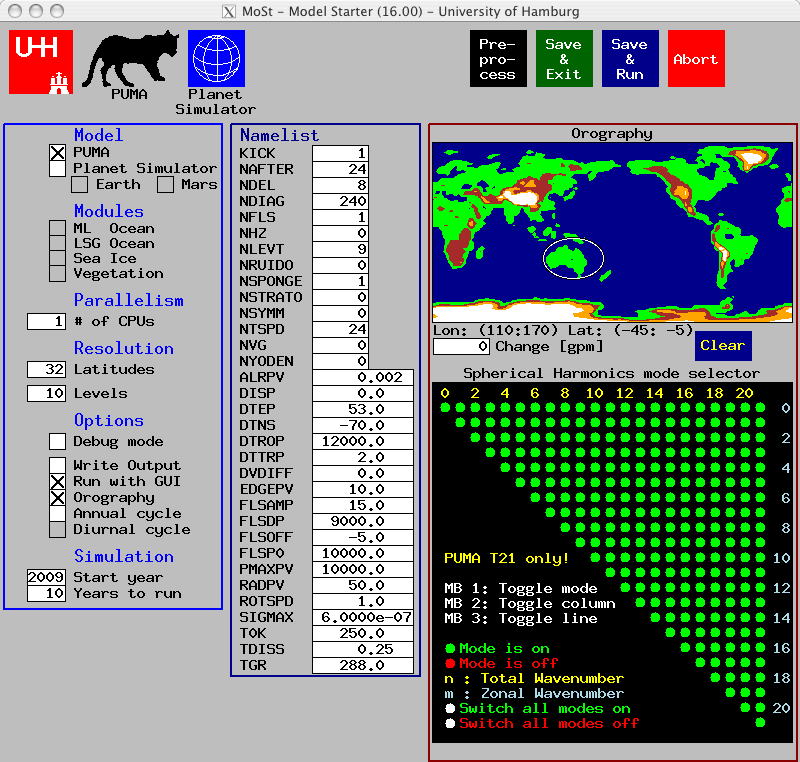
\includegraphics[width=8.5cm]{Pics/mostsnap}
   \caption[]{Screenshot of Model Starter (MoSt)}
   \label{mostsnap}
\end{figure}

The {\model} may be used in the traditional fashion,
with shell scripts, batch jobs, and network queuing 
systems. This is acceptable for long running simulations
on complex machines and number-crunchers, like vector-
computers, massive-parallel-computers and workstation clusters.
There is now, however, a much more convenient method by using
a graphical user interface (GUI) for model setup with parameter configurations
and for interaction between user and model.


The {\model} is configured and setup by the first
GUI module named MoSt (Model Starter, screenshot in \ref{mostsnap}). 
MoSt is the fastest way to get the
model running. It gives access to the most important parameters of
the model preset to the most frequently used values.
The model can be started with a mouse click on the button
labelled "Save \& Run" either with the standard paramater setting
or after editing some of the parameters in the MoSt window.
Some parameters, like horizontal and vertical resolution,
or the number of processors, require the building
(compile, link and load) of new executables. MoSt achieves
this by generating and executing build scripts,
that perform the necessary code changes and
create the required executable.
Other parameters define startup- and
boundary conditions or settings for parameterisations.
They can be edited in MoSt and, after a check for
correct range and consistency with other parameters,
are written to the model's namelist file.

Depending on all settings
MoSt generates a runscript for the simulation.
The user has the choice of leaving MoSt and
continue with the simulation under control of a GUI
right away, or to exit MoSt with the scripts prepared
to run. The second alternative is useful for users, who
want to modify the setup beyond the scope of MoSt
or want to run the Planet Simulator without GUI.

There's also a simple graphical editor for topograpy.
Check the box Orography and then use the mouse to mark
rectangular areas in the topography display.
Enter a value for rising (positive) or lowering the area
and press the button labelled {\bf Preprocess}.
The preprocessor will be built and executed, a new
topography will be computed and written to a start file.

Another editor is the mode editor for spherical harmonics.
Green modes are enabled, red modes are disabled.
This feature can be used to make runs with only certain
modes of spherical harmonics being active.
MB1, MB2, MB3 refer to the left, middle, and right mouse
button. You may toggle individual modes or whole lines
and columns. Currently this mode editor can only be used
for {\model} in the T21 resolution.

\begin{figure}
   \centering
   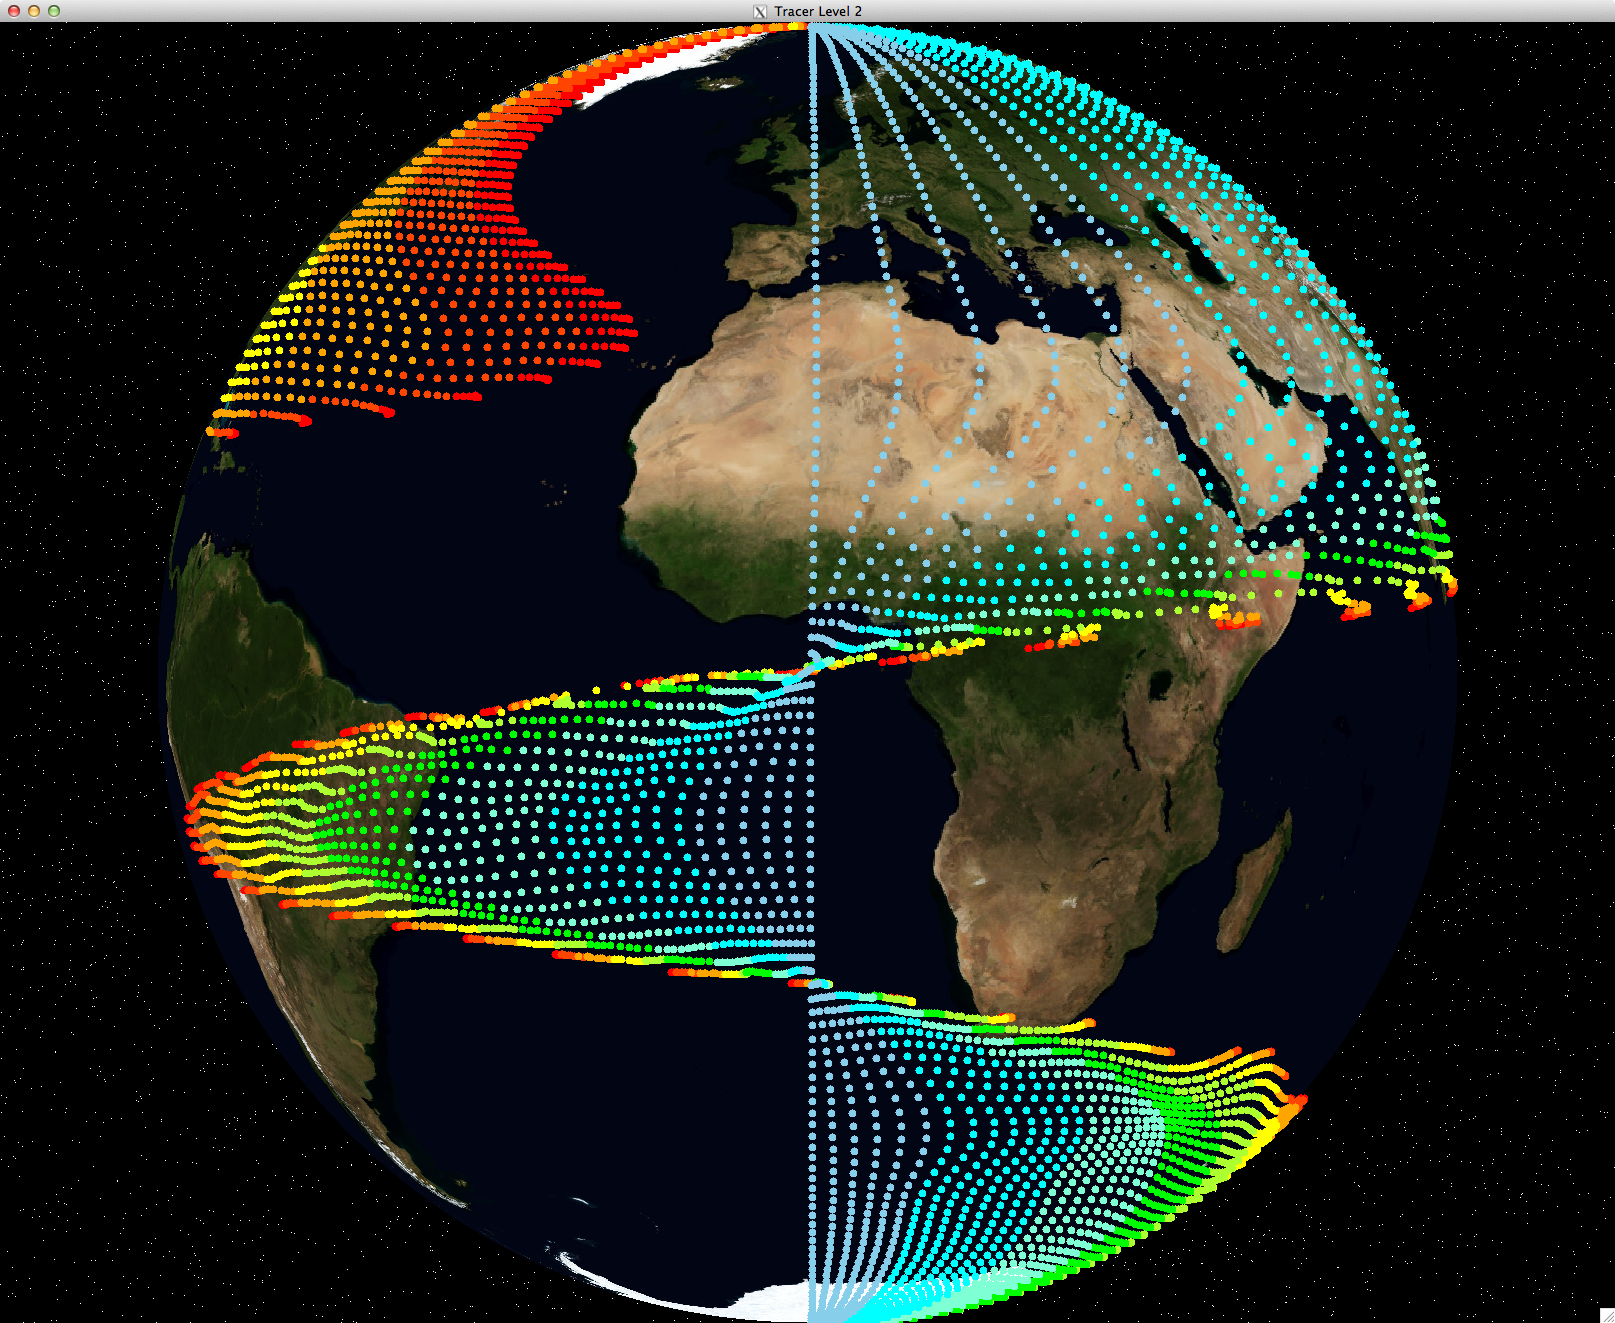
\includegraphics[width=8.5cm]{Pics/guisnap}
   \caption[]{Screenshot of Graphical User Interface (GUI)}
   \label{guisnap}
\end{figure}

The GUI for running the {\model}
(screenshot in \ref{guisnap})
has two main purposes. The first one is to display
model arrays in suitable representations.
Current implementations are:
\begin{itemize}
\item{Zonal mean cross sections}
\item{Horizontal global fields in cylinder projection}
\item{Horizontal global fields in polar projection}
\item{Time-longitude (Hovmoeller) diagrams}
\item{Amplitudes of coefficients of spherical harmonics}
\item{Time series}
\item{Numerical values}
\end{itemize}

In case of horizontal global grids pressing the MMB (Middle Mouse Button)
toggles between cylinder and polar projection. If the grid is
just one level from many of a three dimensional field like u or v,
the level shown can be decreased by the LMB or increased by the RMB.
For Hovmoeller and longitude height sections the LMB and RMB can
be used to select the latitude.

The second purpose is the interaction part of the GUI, which allows the user to change
selected model variables during the model run.
It is not necessary, though possible, to pause the
model while changing variables. Changes to model variables
are, of course, monitored in the outputfile and checked
by GUI for the appropriate range of values and
maximum possible change per timestep because, 
otherwise, a rapid parameter change or a choice of values beyond the normal
range may blow up the model.

All model variables, which are candidates for the display
or interactive changes, have a special code to communicate
with the Planet Simulator. The experienced modeller
can add new code for more variables using the existing
communication code as template. Thus all model fields
or even fields received via coupling with other models
can be put on the GUI display.

Both, MoSt and GUI are implemented using the Xlib (X11R5),
which is a library of routines for graphics and event communication.
As this library is part of every UNIX/Linux operating system
and base of all desktop environments, there is no need
to install additional software for running MoSt and GUI.
Another important  property of Xlib is the full network transparency.
The display of MoSt and GUI is not locked to the machine
running the programs or the model. In fact, the best
performance is obtained in running the Planet Simulator on
two or four CPUs of a remote server while displaying
the GUI on the user's workstation.
In summarizing, the MoSt and GUI programs automate many tedious tasks,
minimize the time to become familiar with the Planet Simulator,
and make debugging and parameter tuning much easier.
More kinds of presentations, coordinate projections
and interactivity are being developed.
A graphical preprocessor with editor for boundary
conditions and a graphical postprocessor are future expansions
to build an almost complete environment for modellers.

\section{GUI configuration}

On initialization the GUI reads its configuration from a file
{\bf GUI.cfg} which must be present in the current directory.
MoSt copies the file {\bf GUI.cfg} from the ../dat/ directory
to the run directory while building the {\model}.
After reading {\bf GUI.cfg} an attempt is made to read the file
{\bf GUI\_last\_used.cfg}. This file is always written at the end
of a GUI controlled simulation. So one may rearrange and position
GUI windows during a run and the new layout will be saved to the
file {\bf GUI\_last\_used.cfg}. In order to make this user
layout default for following runs, just copy this file like:
\begin{verbatim}
Most15/plasim/run$ cp ../dat/GUI.cfg ../dat/GUI.cfg.old
Most15/plasim/run$ cp GUI_last_used.cfg ../dat/GUI.cfg
\end{verbatim}
MoSt will then copy your new layout to the run directory at 
the next invocation.

The {\bf GUI.cfg} is a text file that may be also edited manually.
There is a section for each window (counting from 0 to 8) which
looks like:

\begin{verbatim}
[Window 00]                       <- window number (0..8)
Array:CSU                         <- array name
Plot:ISOCS                        <- picture type
Palette:U                         <- colour palette
Title:Zonal Wind [m/s]            <- window title
Geometry:  529  299    2    3     <- width height left top

[Window 01]
Array:SPAN
Plot:ISOSH
Palette:AMPLI
Title:Spherical Harmonics Ps
Geometry:  529  299  535    3

...

\end{verbatim}

Possible values for these items are:

\subsection{Array}
\begin{tabular}{|l|l|}
\hline
Name     & Description \\
\hline
CSU      & Cross Section U - Zonal mean zonal wind \\
CSV      & Cross Section V - Zonal mean meridional wind \\
CST      & Cross Section T - Zonal mean temperature \\
SPAN     & Spherical harmonics coefficients of surface pressure \\
GU       & Three dimensional grid of zonal wind \\
GV       & Three dimensional grid of meridional wind \\
GP       & Grid of surface pressure \\
DQVI     & Vertically integrated humidity \\
GUCOL    & sounding of eastward wind at a grid point \\
GVCOL    & sounding of northward wind a grid point \\
GTCOL    & sounding of temperature at a grid point \\
DQCOL    & sounding of humidity at a grid point \\
DQLCOL   & sounding of liquid water at a grid point \\
DCCCOL   & sounding of cloud cover at a grid point \\
SCALAR   & Selected scalars for timeseries and tables \\
\hline
\end{tabular}

\subsection{Plot}
\begin{tabular}{|l|l|}
\hline
Name     & Description \\
\hline
   ISOHOR & Isolines and colouring of horizontal grids \\
   ISOCS &  Isolines and colouring of cross sections \\
   ISOHOV & Colouring of Hovmoeller diagram \\
   ISOTS &  Timeseries \\
   ISOTAB & Tables \\
   ISOSH &  Coloured amplitudes \\
   ISOLON & Isolines and colouring of longitude height section \\
   ISOCOL & vertical Hovmoeller diagram for soundings \\
\hline
\end{tabular}

\subsection{Palette}
\begin{tabular}{|l|l|l|}
\hline
Name     & Range & Description  \\
\hline
   AUTO & automatic & rainbow colours \\
   U &    -10 .. 50 & rainbow colours \\
   V &    -10 .. 10 & rainbow colours \\
   T &    -50 .. 50 & blue - red \\
   P &    985 .. 1025 & blue - red \\ 
   Q &      0 .. 60 & rainbow colours \\
   DCC   &  0 ..100 & rainbow colours \\
   MARST & -90 .. 0 & blue -red \\
   AMPLI & 0 .. 12 & blue - green -red \\
   VEG   & 0 .. 100 & shades of green \\
\hline
\end{tabular}

\subsection{Title}
The title item may contain any text, but keep it short,
the length of the window's title bar is limited.
The words {\em Latitude} and {\em Level} have special
features in conjunction with threedimensional arrays,
where the user may scroll the level or latitude.
The GUI will insert the level number after the world 
{\em Level} or the latitude after the word {\em Latitude}.

\subsection{Geometry}
The four integers following the geometry item describe
the size and screen position of the window.
The first two parameters refer to width and height in 
screen pixel. These are the sizes of the inner window,
title bar, border and other decorations are not counted.
The third and fourth parameter set the coordinates of the
upper left corner of the window x and y, again without borders.
If the geometry item is not defined, the GUI will
initialize the window's geometry depending on the screen size.




\chapter{Postprocessor Pumaburner}
\label{Pumaburner}
\section{Introduction}

The {\bf Pumaburner} is a postprocessor for the {\bf Planet Simulator}
and the {\bf PUMA} model family.
It's the only interface between {\it raw} model data output
and diagnostics, graphics, and user software.

The output data of the {\bf Planet Simulator} are stored as
packed binary (16 bit) values using the model representation.
Prognostic variables like temperature, divergence, vorticity,
pressure, and humidity are stored as coefficients of spherical harmonics
on $\sigma$ levels. Variables like radiation,
precipitation, evaporation, clouds, and other fields of the
parameterization package are stored on Gaussian grids.

The tasks of the {\bf Pumaburner} are:
\begin{itemize}
\item Unpack the {\it raw} data to full real representation.
\item Transform variables from the model's representation
      to a user selectable format, e.g. grids,
      zonal mean cross sections, fourier coefficients.
\item Calculate diagnostic variables, like vertical velocity,
      geopotential height, wind components, etc.
\item Transfrom variables from $\sigma$ levels to user
      selectable pressure levels.
\item Compute monthly means and standard deviations.
\item Write selected data either in SERVICE, GRIB, or NetCDF format
      for further processing.
\end{itemize}

\section{Usage}

\begin{verbatim}
pumaburn4 [options] InputFile OutputFile <namelist >printout
     option -h : help (this output)
     option -c : print available codes and names
     option -d : debug mode (verbose output)
     option -g : Grib   output (override namelist option)
     option -n : NetCDF output (override namelist option)
     option -m : Mean=1 output (override namelist option)
     InputFile : Planet Simulator or PUMA data file
    OutputFile : GRIB, SERVICE, or NetCDF format file
      namelist : redirected <stdin>
      printout : redirected <stdout>
\end{verbatim}

\section{Namelist}

The namelist values control the selection, coordinate system
and output format of the postprocessed variables.
Names and values are not case sensitive.
You can assign values to the following names: \vspace{0.4cm}

\begin{tabular}{|l|c|l|l|l|}
\hline
Name   & Def. & Type & Description & Example \\
\hline
{\bf HTYPE  }& S & char & Horizontal type               & HTYPE=G \\
{\bf VTYPE  }& S & char & Vertical type                 & VTYPE=P \\
{\bf MODLEV }& 0 & int  & Model levels                  & MODLEV=2,3,4 \\
{\bf hPa    }& 0 & real & Pressure levels               & hPa=500,1000 \\
{\bf CODE   }& 0 & int  & ECMWF field code              & CODE=130,152 \\
{\bf GRIB   }& 0 & int  & GRIB output selector          & GRIB=1 \\
{\bf NETCDF }& 0 & int  & NetCDF output selector        & NETCDF=1 \\
{\bf MEAN   }& 1 & int  & Compute monthly means         & MEAN=0 \\
{\bf HHMM   }& 1 & int  & Time format in Service format & HHMM=0 \\
{\bf HEAD7  }& 0 & int  & User parameter                & HEAD7=0815 \\
{\bf MARS   }& 0 & int  & Use constants for planet Mars & MARS=1 \\
{\bf MULTI  }& 0 & int  & Process multiple input files  & MULTI=12 \\
\hline
\end{tabular}

\section{HTYPE}

{\bf HTYPE} accepts the first character of the following string.
Following settings are equivalent: HTYPE = S, HTYPE=Spherical Harmonics
HTYPE = Something. Blanks and the equal-sign are optional. \\
Possible Values are:

\begin{tabular}{|l|l|l|}
\hline
   Setting   & Description          & Dimension for T21 resolution   \\
\hline
   HTYPE = S & Spherical Harmonics  & (506):(22 * 23 coefficients)   \\
   HTYPE = F & Fourier Coefficients & (32,42):(latitudes,wavenumber) \\
   HTYPE = Z & Zonal Means          & (32,levels):(latitudes,levels) \\
   HTYPE = G & Gauss Grid           & (64,32):(longitudes,latitudes) \\
\hline
\end{tabular}

\section{VTYPE}

{\bf VTYPE} accepts the first character of the following string.
Following settings are equivalent: VTYPE = S, VTYPE=Sigma
VTYPE = Super. Blanks and the equal-sign are optional. \\
Possible Values are:

\begin{tabular}{|l|l|l|}
\hline
   Setting   & Description          & Remark \\
\hline
   VTYPE = S & Sigma (model) levels & Some derived variables are not available \\
   VTYPE = P & Pressure levels      & Interpolation to pressure levels \\
\hline
\end{tabular}

\section{MODLEV}

{\bf MODLEV} is used in combination with {\bf VTYPE = S}.
If VTYPE is not set to Sigma, the contents of MODLEV are ignored.
MODLEV is an integer array that can get as many values as there are
levels in the model output. The levels are numbered from top of
the atmosphere to the bottom. The number of levels and the 
corresponding sigma values are listed in the pumaburner printout.
The outputfile orders the level according to the MODLEV values.
MODLEV=1,2,3,4,5 produces an output file of five model levels
sorted from top to bottom, while MODLEV=5,4,3,2,1 sorts them
from bottom to top.

\section{hPa}

{\bf hPa} is used in combination with {\bf VTYPE = P}.
If VTYPE is not set to Pressure, the contents of hPa are ignored.
hPa is a real array that accepts pressure values with the
units hectoPascal or millibar. All output variables will be
interpolated to the selected pressure levels.
There is no extrapolation on the top of the atmosphere.
For pressure values, that are lower than that of the model's
top level, the top level value of the variable is taken.
The variables temperature and geopotential height are extrapolated
if the selected pressure is higher than the surface pressure.
All other variables are set to the value of the lowest mode level
for this case. The outputfile contains the levels in the same order
as set in hPa. Example: hpa = 100,300,500,700,850,900,1000.

\section{MEAN}

{\bf MEAN} can be used to compute montly means and/or deviations.
The Pumaburner reads date and time information from the model file
and handles different lengths of months and output intervals correctly.

\begin{tabular}{|l|p{12cm}|}
\hline
Setting & Description \\
\hline
        MEAN  =  0 & Do no averaging - all terms are processed. \\

        MEAN  =  1 & Compute and write monthly mean fields.
                     Not for spherical harmonics, Fourier coefficients or
                     zonal means on sigma levels. \\

        MEAN  =  2 & Compute and write monthly deviations.
                     Not for spherical harmonics, Fourier coefficients or
                     zonal means on sigma levels.
                     Deviations are not available for NetCDF output. \\

        MEAN  =  3 & Combination of MEAN=1 and MEAN=2.
                     Each mean field is followed by a deviation
                     field with an identical header record.
                     Not for spherical harmonics, Fourier coefficients or
                     zonal means on sigma levels. \\
\hline
\end{tabular}

\section{Format of output data}

The {\bf pumaburner} supports three different output formats:

\begin{itemize}
\item {\bf GRIB} (GRIdded Binary) WMO standard for gridded data.
\item {\bf NetCDF} (Network Common Data Format)
\item {\bf Service} Format for user readable data (see below).
\end{itemize}

For more detailed descriptions see for example:

{\url{http://www.nws.noaa.gov/om/ord/iob/NOAAPORT/resources/}}

\begin{tabular}{|l|l|p{10cm}|}
\hline
Setting & Description \\
\hline
   GRIB = 1 & NetCDF = 0 & The output file is written GRIB format.
                     This option can be used only for
                     HTYPE=Spherical Harmonics or HTYPE=Gauss Grid. \\
   GRIB = 0 & NetCDF = 1 & The output file is written in NetCDF format.
                     This option can be used for HTYPE=Gauss Grid only. \\
   GRIB = 0 & NetCDF = 0 & The output file is written in Service format.
                     This is the preferred format for user programs.
                     For a detailed description see the following section. \\
   GRIB = 1 & NetCDF = 1 & Illegal combination. \\
\hline
\end{tabular}

\section{SERVICE format}

     The SERVICE format uses the following structure:
     The whole file consists of pairs of
     header records and data records.
     The header record is an integer array of 8 elements.

\begin{verbatim}
     head(1) = ECMWF field code
     head(2) = modellevel or pressure in [Pa]
     head(3) = date  [yymmdd]  (yymm00 for monthly means)
     head(4) = time  [hhmm]  or [hh] for HHMM=0
     head(5) = 1. dimension of data array
     head(6) = 2. dimension of data array
     head(7) = may be set with the parameter HEAD7
     head(8) = experiment number (extracted from filename)

     Example for reading the SERVICE format (GRIB=0 , NETCDF=0)

     INTEGER HEAD(8)
     REAL    FIELD(64,32)     ! dimensions for T21 grids
     READ (10,ERR=888,END=999) HEAD
     READ (10,ERR=888,END=999) FIELD
     ....
 888 STOP 'I/O ERR'
 999 STOP 'EOF'
     ....
\end{verbatim}

\section{HHMM}

\begin{tabular}{|l|p{12cm}|}
\hline
Setting & Description \\
\hline
  HHMM  =  0 & head(4) shows the time in hours (HH). \\
  HHMM  =  1 & head(4) shows the time in hours and minutes (HHMM). \\
\hline
\end{tabular}

\section{HEAD7}
The 7th. element of the header is reserved for the user.
It may be used for experiment numbers, flags or anything else.
Setting HEAD7 to a number exports this number to every header record
in the output file (SERVICE format only).

\section{MARS}
This parameter is used for processing simulations of the Mars atmosphere.
Setting MARS=1 switches gravity, gas constant and planet radius
to the correct values for the planet Mars.

\section{MULTI}
The parameter MULTI can bes used to process a series of input data
within one run of the pumaburner. Setting MULTI to a number (n)
tells the pumaburner to procees (n) input files.
The input files must follow one of the following two rules:
\begin{itemize}
\item YYMM rule: The last four characters of the filename 
                 contain the data in the form YYMM.
\item .NNN rule: The last four characters of the filename
                 consist of a dot followed ny a 3-digit sequence number.
\end{itemize}

\begin{verbatim}
Examples:

Namelist contains MULTI=3
Command: pumaburn <namelist >printout run.005 out
pumaburn processes the files <run.005> <run.006> <run.007>

Namelist contains MULTI=4
Command: pumaburn <namelist >printout exp0211 out
pumaburn processes the files <exp0211> <exp0212> <exp0301> <exp0302>
\end{verbatim}

\section{Namelist example}
\begin{verbatim}
       VTYPE  = Pressure
       HTYPE  = Grid
       CODE   = 130,131,132
       hPa    = 200,500,700,850,1000
       MEAN   = 0
       GRIB   = 0
       NETCDF = 0
\end{verbatim}

    This namelist will write Temperature(130), u(130) and v(131)
    on pressure levels 200hPa, 500hPa, 700hPa, 850hPa and 1000hPa.
    The output interval is the same as found on the model data,
    e.g. every 12 or every 6 hours (MEAN=0). The output format
    is SERVICE format.

\section{Troubleshooting}
If the pumaburner reports an error or doesn't produce 
the expected results, try the following:

\begin{itemize}

\item Check your namelist, especially for invalid codes, types and levels.

\item Run the pumaburner in debug-mode by using the option -d.
Example:
\begin{verbatim}
pumaburn <namelist >printout -d data.in data.out
\end{verbatim}

This will print out some details like parameters and memory allocation
during the run. The additional information may help to detect
the problem.

\item Not all combinations of HTYPE, VTYPE, and CODE are valid.
Try to use HTYPE=Grid and VTYPE=Pressure before switching to
exotic parameter combinations.

\end{itemize}



\chapter{Graphics}
%\section{\verb/GrADS/}
\section{GrADS}
In this section, visualisation using the graphics package \verb#GrADS#
({\bf Gr}id {\bf A}nalysis and {\bf D}isplay {\bf S}ystem) is
described. A useful Internet site for reference and for installation
instructions is
\begin{quote}
{\url{http://grads.iges.org/grads/grads.html}}.
\end{quote}
The latest version of \verb#GrADS# can handle data in \verb#NetCDF#
format via the command \verb#sdfopen#.
Any file produced by the \verb#Pumaburner# with the option NETCDF=1
can be read directly by \verb#GrADS#.
For files in the \verb#SERVICE# format is possible to use
a converter, which translates from the \verb#SERVICE# format into \verb#NetCDF#.
But in the following it is assumed that the \verb/PUMA/ output has been
postprocessed into the \verb#SERVICE# format with the \verb#Pumaburner# and that the
resulting file is called \verb/puma.srv/. Using the option -g for the \verb#Pumaburner# 
creates the related GrADS control file \verb/puma.ctl/.
Monthly mean data is either obtained
directly from the \verb#Pumaburner# (\verb#namelist# parameter
\verb#MEAN=1#, see section \ref{Pumaburner}) or via a
\verb/CDO/ command:
\begin{quote}
\verb/cdo monmean puma.srv puma_m.srv/
\end{quote}
\noindent Information on the {\bf C}limate {\bf D}ata {\bf O}perators ({\bf CDO}'s)
can be found in the \verb#CDO User's Guide# at
\begin{quote}
 {\url{http://www.mpimet.mpg.de/fileadmin/software/cdo/}}.
\end{quote}
When the \verb#GrADS# control file was not created via the \verb#Pumaburner# 
option -g, it can be done by the command:

\begin{quote}
\verb#srvctl puma_m.srv#
\end{quote}
\noindent which creates the file \verb/puma_m.ctl/. 
It contains information on the grid, time steps, and variable names. The file
\verb/puma_m.srv/ is still needed in addition.
The program
\verb#srvctl.f90# is one of the post-processing tools available at
\begin{quote}
{\url{http://mi.uni-hamburg.de/puma/}}.
\end{quote}
If you chose to compile it yourself, please read the comments in the
first few lines of the program text. Sometimes the
\verb/srvctl/ tool has difficulty calculating an appropriate time axis 
from the data headers of the data records, so you should check this. 
In particular the number of days per year is concerned: \verb#GrADS# may assume 365
days per year even though the data header says 360 days per year.
This is an example of what the \verb/puma_m.ctl/ should look like:
\begin{verbatim}
DSET ^puma_m.gra
UNDEF 9e+09
XDEF     64 LINEAR   0.0000   5.6250
OPTIONS YREV
YDEF     32 LEVELS 
  -85.7606  -80.2688  -74.7445  -69.2130  -63.6786  -58.1430  -52.6065  -47.0696
  -41.5325  -35.9951  -30.4576  -24.9199  -19.3822  -13.8445   -8.3067   -2.7689
    2.7689    8.3067   13.8445   19.3822   24.9199   30.4576   35.9951   41.5325
   47.0696   52.6065   58.1430   63.6786   69.2130   74.7445   80.2688   85.7606
ZDEF      5 LEVELS 
     20000
     50000
     70000
     85000
    100000
TDEF 12 LINEAR 00:00Z01jan0001        1mo
VARS  3
c130     5 99    130     0     0
c131     5 99    131     0     0
c132     5 99    132     0     0
ENDVARS
\end{verbatim}
Here, since we are handling monthly mean data, the line starting 
with \verb/TDEF/ ends with \verb/1mo/. When the \verb/PUMA/ output is used
without averaging, this should correspond to the output interval given
by the \verb#nwpd# variable used in the \verb#namelist# of your \verb#PUMA#
run (see Appendix \ref{Namelist}). The number of variables
depends on how the Pumaburner was
called. In this example, only three variables were processed, i.e.\ the
temperature (\verb/c130/), the zonal wind (\verb/c131/) and the meridional 
wind (\verb/c132/). Refer to Appendix \ref{Pumacodes} for a list of the codes.
\\
The GrADS program is started by typing \verb/grads/ in a terminal window. 
Then, the data is displayed either by typing commands line-by-line, 
or preferably by using scripts. The following script, called \verb/tglob.gs/, 
displays the monthly mean temperature at 500hPa:
\begin{verbatim}
# tglob.gs
function pass(m)
'reinit'
'open puma_m'
'enable print print.mf'
'set t 'm
'set lev 50000'
'c'
'set gxout shaded'
'd (c130-273.16)'
'cbar.gs'
'set gxout contour'
'd (c130-273.16)'
'draw title Temperature (deg C) 500hPa month 'm
'print'
'disable print'
'!gxps -i print.mf -o tglob'm'.ps'
\end{verbatim}
The variable \verb/m/ at the beginning of the script defines the month 
which should be displayed. It is passed from the terminal with the 
script call. Note that no quotation marks are present in this line, 
since only \verb/GrADS/ specific commands are framed by quotation marks. 
Script commands, variable definitions, if-clauses, etc. are used without 
quotation marks. The script is executed by typing its name, without 
the suffix \verb/.gs/, followed by the number of the month to be shown. 
For example, \verb/tglob 7/ displays the monthly mean temperature at 500hPa
in July. The resulting output file is called \verb/tglob7.ps/. 
\par
\vspace{3mm}
The following script \verb/thh/ displays the time dependent 
temperature (in 1000hPa) of Hamburg. Here, two variables are passed to \verb/GrADS/ to plot, 
the first day and the last day. (Note that here, the file \verb/puma.gra/ 
is opened, which contains data on a daily basis). The call \verb/thh 91 180/ 
displays the temperature in 1000hPa of Hamburg for the spring season 
from April 1st to June 30th.

\begin{verbatim}
# thh.gs
function pass(d1 d2)
'reinit'
'open puma'
'enable print print.mf'
'set lat 53'
'set lon 10'
'set lev 100000'
'set t 'd1' 'd2
'c'
'd (c130-273.16)'
'draw title Temperature (deg C) 1000hPa in Hamburg'
'print'
'disable print'
'!gxps -i print.mf -o thh.ps'
\end{verbatim}

\vspace{3mm}
It is possible to have more than one figure in a plot, which is 
illustrated in the following script. It plots the seasonal means 
of the sea level pressure. The data file is prepared like this:

\begin{verbatim}
cdo selcode,151 puma.srv slp.srv    #code 151 has to be in puma.srv  
cdo seasmean slp.srv slp_sm.srv
srv2gra slp_sm.srv
\end{verbatim}

The command \verb/set vpage/ sets a virtual page inside the graphic 
window. The full window is 11 inch wide and 8.5 inch high, so 
\verb/set vpage 0 5.5 4.25 8.5/ defines the upper left corner. 
If \verb/setlevs=1/ is specified, then the pressure levels as given are used. 
Otherwise, \verb/GrADS/ defines contour levels depending on the data set.

\begin{verbatim}
# slp_sm.gs
setlevs=1
'reinit'
'open slp_sm'
'enable print print.mf'
'c'
'set vpage 0 5.5 4.25 8.5'
'set gxout contour'
if (setlevs=1)
'set clevs 990 995 1000 1005 1010 1015 1020'
endif
'set ccols 1'
'set grads off'
'set t 1'
'd c151/100'
'draw title SLP [hPa] yr 'ny' DJF'
'set vpage 5.5 11 4.25 8.5'
'set gxout contour'
if (setlevs=1)
'set clevs 990 995 1000 1005 1010 1015 1020'
endif
'set ccols 1'
'set grads off'
'set t 2'
'd c151/100'
'draw title yr 'ny' MAM'
'set vpage 0 5.5 0 4.25'
'set gxout contour'
if (setlevs=1)
'set clevs 990 995 1000 1005 1010 1015 1020'
endif
'set ccols 1'
'set grads off'
'set t 3'
'd c151/100'
'draw title yr 'ny' JJA'
'set vpage 5.5 11 0 4.25'
'set gxout contour'
if (setlevs=1)
'set clevs 990 995 1000 1005 1010 1015 1020'
endif
'set ccols 1'
'set grads off'
'set t 4'
'd c151/100'
'draw title yr 'ny' SON'
'print'
'disable print'
'!gxps -c -i print.mf -o slp_sm.ps'
\end{verbatim}

%\section{Vis5D}
%\begin{quote}
{\it ``Vis5D is a system for interactive visualization of large 5-D
gridded data sets such as those produced by numerical weather
models. One can make isosurfaces, contour line slices, colored slices,
volume renderings, etc of data in a 3-D grid, then rotate and animate
the images in real time. There's also a feature for wind trajectory
tracing, a way to make text annotations for publications, support for
interactive data analysis, etc.''}
\par
\end{quote}
\begin{flushright}
from the Vis5D home page,\\
{\url{http://www.ssec.wisc.edu/~billh/vis5d.html}}
\end{flushright}
\par
\noindent This powerful visualisation tool together with its documentation is
available through the above home page. Vis5D uses its own data format
which makes it necessary to transform your data. Depending on their
format
% (see also section \ref{Filestructure}
 and the flowchart on
{\url{http://puma.dkrz.de/puma/download/map/}} you have the following
choices: If

\begin{itemize}
\item{{\it your data is raw \verb#PUMA# output,}\\
	you need to process it with the \verb#pumaburner#
	postprocessor (see section \ref{Pumaburner}) in order to
	transform it to either
	\verb#NETCDF#} (option \verb#-n# or namelist parameter
	\verb#NETCDF=1#) or \verb#GRIB# (option \verb#-g# or namelist
	parameter \verb#GRIB=1#) and proceed from there.
\item{{\it your data is in \verb#SERVICE# format,}\\
	you need to convert it to either \verb#GRIB#, for
	instance with the \verb#PINGO#s:
\begin{quote}
 \verb#grb copy2 data.srv data_with_grib_metainfo.grb output.grb#,
\end{quote}	
	or \verb#NETCDF#,
	using the program \verb#puma2cdf#, which is available with the
	\verb#PUMA# postprocessing tools. Despite of its name this
	program cannot process raw \verb#PUMA# output but takes
	\verb#SERVICE# format as input. It can as well be called as
	\verb#srv2cdf# which changes its behaviour: oddities of model
	output such as the existence of February, $30^{th}$ are
	then no longer removed.	Once the format is changed proceed from there.}
\item{{\it your data is in \verb#NETCDF# format,}\\
	it can easily transformed to \verb#Vis5D#'s native format by
	means of the program \verb#cdf2v2d#, which is available with
 	the \verb#PUMA# postprocessing tools.}
\item{{\it your data is in \verb#GRIB# format,\\}
	you can find a transformation tool named \verb#Grib2V5d# at\\
	\verb#<http://grib2v5d.sourceforge.net># which offers various
	practical features.}
\end{itemize}
\noindent Once the conversion to \verb#Vis5D#'s native format is
	achieved please follow the instructions from the \verb#Vis5D#
	documentation or, if \verb#Vis5D# is already installed on your
	system, try finding your own way by typing:
\begin{quote}
\verb#vis5d my_data.v5d#
\end{quote}



\chapter{Model Dynamics}
\section{Model equations and numerics}

The core of the model is a set of primitive equations. They describe
the conservation of momentum, mass, and thermal energy.
Using spherical coordinates and the sigma system and with
the aid of the equation of state they can be written in the
dimensionless form as follows:

{\bf Conservation of momentum:}

Vorticity equation
\begin{equation}
\pd{(\zeta + f)}{t} = \frac{1}{(1-\mu^2)}\pd{F_v}{\lambda}-\pd{F_u}{\mu}+P_{\zeta}
\label{vortgl}
\end{equation}
Divergence equation
\begin{equation}
\pd{D}{t} = \frac{1}{(1-\mu^2)}\pd{F_u}{\lambda}+\pd{F_v}{\mu}-\nabla^2\left(\frac{U^2+V^2}{2(1-\mu^2)}+\Phi+T_0\ln p_s\right)+P_D
\label{divgl}
\end{equation}
Hydrostatic approximation
\begin{equation}
\pd{\Phi}{\ln\sigma} = -T
\label{hydrogl}
\end{equation}
{\bf Conservation of mass:}

Continuity equation
\begin{equation}
\pd{\ln p_s}{t} = -\int\limits_0^1Ad\sigma
\label{kontigl}
\end{equation}
{\bf Conservation of energy:}

First law of thermodynamics
\begin{equation}
\pd{T'}{t} = -\frac{1}{(1-\mu^2)}\pd{(UT')}{\lambda}-\pd{(VT')}{\mu}+DT'-\dot{\sigma}\pd{T}{\sigma}+\kappa\frac{T}{p}\omega+\frac{J}{c_p}+P_T,
\label{thermogl}
\end{equation}
with:

\bfl
$ \di F_u = V(\zeta+f)-\dot{\sigma}\pd{U}{\sigma}-T'\pd{\ln p_s}{\lambda} $
\efl
\bfl
$ \di F_v = -U(\zeta+f)-\dot{\sigma}\pd{V}{\sigma}-T'(1-\mu^2)\pd{\ln p_s}{\mu} $
\efl
\bfl
$ \di A = D+\vec{V}\cdot\nabla\ln p_s $
\efl
and \quad $U = u\cos\phi$, $V = v\cos\phi$.

Where the variables denote:
\begin{tabbing}
xxxxxxxxxxxxxxxxx\=xxxxxxxxxxxxxxxxxxxxxxxxxxxxxxxxxxxxxxx\kill
$T$ \> temperature \\
$T_0$ \> reference temperature \\
$T'=T-T_0$ \> temperature deviation from $T_0$ \\
$\zeta$ \> relative vorticity \\
$D$ \> divergence \\
$p_s$ \> surface pressure \\
$p$ \> pressure \\
$\Phi$ \> geopotential \\
$t$ \> time \\
$\lambda$, $\phi$ \> longitude, latitude \\
$\mu=\sin\phi$ \> \\
$\sigma=p/p_s$ \> sigma vertical coordinate \\
$\dot{\sigma}=d\sigma/dt$ \> vertical velocity in $\sigma$-system \\
$\omega=dp/dt$ \> vertical velocity in $p$-system \\
$u$, $v$ \> zonal, meridional component of horizontal velocity \\
$\vec{V}$ \> horizontal velocity with components $U$, $V$ \\
$f$ \> Coriolis parameter \\
$J$ \> diabatic heating rate \\
$c_p$ \> specific heat of dry air at constant pressure \\
$\kappa$ \> adiabatic coefficient \\
\end{tabbing}
The set of differential equations consists of the four prognostic
equations (\ref{vortgl}), (\ref{divgl}), (\ref{kontigl}), and
(\ref{thermogl}). Vorticity $\zeta$ and divergence $D$ are
scaled by the angular velocity of the earth $\Omega$, pressures $p$
and $p_s$ are scaled by the global mean surface pressure $P_s=1011\,hPa$,
temperatures $T$ and $T_0$ are scaled by $a^2\Omega^2/R$, geopotential
$\Phi$ is scaled by $a^2\Omega^2/g$, and time $t$ is scaledby $\Omega^{-1}$, where
$a$ is the radius of the earth, $R$ is the gas constant of dry air,
and $g$ is the gravitational acceleration.
For the parameterizations $P_\zeta$, $P_D$ and $P_T$ see section
\ref{parametrisierungen}. The model can be run with or without orography.

The horizontal representation of any model variable is given
by a series of spherical harmonics. If $Q$ is an arbitrary
model variable, then its spectral representation has the form:
\begin{equation}
\label{spektral}
Q(\lambda,\mu,t) = \sum_\gamma Q_\gamma(t)\,Y_\gamma(\lambda,\mu).
\end{equation}
Here, $Y_\gamma$ are the spherical harmonics, and $Q_\gamma$ the
corresponding complex amplitudes, where $\gamma=(n,m)$ designates
the spectral modes ($n=1,\,2,\,3,\ldots$: total wave number;
$m=0,\,\pm1,\,\pm2,\,\pm3,\ldots$: zonal wave number),
with $|m|\le n$ \citep{holton}. The latter condition follows
from the triangular truncation in wave number space.
The truncation is done at the total wave number $n_T$, which
can be set to $n_T=21,31,42,85,127,170$, i.e. the model can be
used with the T21,\ldots,T170 spectral resolution. The vertical
resolution is given by $n_L$ equidistant $\sigma$-levels with the
standard value $n_L=5$. At the upper ($\sigma=0$) and lower boundary
($\sigma=1$) of the model domain the vertical velocity is set to zero
($\dot{\sigma}=0$).

The linear contributions to the tendencies are calculated in the spectral 
domain, the nonlinear contributions in grid point space. Therefore, at 
every time step, the necessary model variables are transformed from 
spectral to grid point representation by Legendre and Fast Fourier (FFT)
transformations, and then the calculated tendencies are transformed back 
into the spectral domain where the time step is carried out 
\citep[for the transform method see][]{orszag70, eliasen70}. Because of 
the semi-implicit time integration scheme \citep*{hossim75, simhosburr78} 
the terms due to gravity wave propagation are integrated in time implicitly, 
and the remaining terms are integrated explicitly, the latter with a 
leap-frog time step. In the standard model, a time step of one hour is used. 
A Robert-Asselin time filter \citep*{halwilli} is applied to avoid decoupling 
of the two leap-frog time levels. The contributions to the tendencies due 
to vertical advection are calculated by an energy and angular-momentum 
conserving vertical finite-difference scheme \citep*{simburr81}.

\section{Parameterizations}
\label{parametrisierungen}

\subsection{Friction}

The dissipative processes in the atmosphere are parameterized using a linear 
approach (Rayleigh friction), which describes the effects of surface drag and 
vertical transport of the horizontal momentum due to small scale turbulence 
in the boundary layer. To achieve this, vorticity $\zeta$ and divergence $D$ 
are damped towards the state of rest ($\zeta=0,\,D=0$) with the time scale $\tau_F$.

The parameterization terms $P_\zeta$ and $P_D$ appear in the model equations 
(\ref{vortgl}) resp. (\ref{divgl}) and have the form:
\beqa
P_\zeta & = & \frac{\zeta}{\tau_F}+H_\zeta \label{paraz} \\
P_D & = & \frac{D}{\tau_F}+H_D. \label{parad}
\eeqa
The time scale $(\tau_F)_l$ depends on the $\sigma$-level $l$ ($l=1,\ldots,n_l$). 
Usually, for the upper levels ($l=1,\ldots,n_l-1$) it is set to 
$(\tau_F)_l=\infty$ (no friction) and for the lowest level ($l=n_l$) 
a typical value is $(\tau_F)_l=1\,d$. An explanation of the hyperdiffusion terms 
$H_\zeta$ and $H_D$ follows in section \ref{diffusion}.

\subsection{Diabatic heating}
\label{diabatischeheizung}

All the diabatic processes considered in the model are also parameterized using 
a linear approach (Newtonian cooling). They include the diabatic heating due to 
absorption and emission of short and long wave radiation, as well as latent and 
sensible heat fluxes (convection). The temperature $T$ relaxes towards the 
restoration temperature $T_R$ with the time scale $\tau_R$. The parameterization 
term in the thermal energy equation (\ref{thermogl}) is given by:
\begin{equation}
\frac{J}{c_p}+P_T = \frac{T_R-T}{\tau_R}+H_T. \label{parat}
\end{equation}
For the hyperdiffusion $H_T$ see section \ref{diffusion}. $\tau_R$ depends on 
the $\sigma$-level $l$, $T_R$ on the latitude $\phi$ and on the vertical 
coordinate $\sigma$. The restoration temperature field has the form:
\begin{equation}
\label{glgTr_2d}
T_R(\phi,\sigma) = T_R(\sigma)+f(\sigma)\,T_R(\phi).
\end{equation}

The vertical profile is described by:
\begin{equation}
T_R(\sigma) = (T_R)_{tp}+\sqrt{\left[\frac{L}{2}\Big(z_{tp}-z(\sigma)\Big)\right]^2+S^2}\,+\,\frac{L}{2}\Big(z_{tp}-z(\sigma)\Big),
\end{equation}
with $\di (T_R)_{tp}=(T_R)_{grd}-L\,z_{tp}$. Here, $z$ denotes the geometric 
height, $z_{tp}$ the global constant height of the tropopause, 
$L=-(\partial T_R)/(\partial z)$ the vertical restoration temperature gradient, 
$(T_R)_{grd}$ and $(T_R)_{tp}$ the restoration temperature at the surface and at 
the global isothermal tropopause, respectively. $S$ provides a smoothing of the 
profile at the tropopause. $z(\sigma)$ is determined by an iterative method. 
The profile is determined by setting the parameters $(T_R)_{grd}$, $z_{tp}$, 
$L$ and $S$.  Figure \ref{Tr_z} shows the vertical profile for the standard 
parameter values.

% 37.4.09: erscheint so im naechsten Abschnitt: \begin{figure}[!!!b]
\begin{figure}[h]
\begin{minipage}{.5\linewidth}
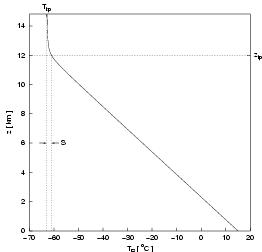
\includegraphics{Pics/Tr_z_Eng}
%\centering \epsfig{figure=Tr_z.Eng.eps, width=\linewidth}
\end{minipage}
\begin{minipage}{.5\linewidth}
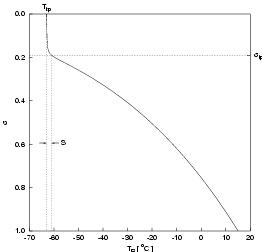
\includegraphics{Pics/Tr_sigma_Eng}
%\centering \epsfig{figure=Tr_sigma.Eng.eps, width=\linewidth}
\end{minipage}
\caption{\footnotesize{Vertical profile of the restoration temperature $T_R$ as 
function of the geometric height $z$ (left) and as function of the dimensionless 
vertical coordinate $\sigma$ (right) for standard parameter values: 
$(T_R)_{grd}=288\,K$; $z_{tp}=12\,km$; $L=6.5\,K/km$; $S=2\,K$.}} \label{Tr_z}
\end{figure}

The temperature contrast between low and high latitudes due to the differential 
radiative energy balance, which drives the general circulation, is described by 
the meridional form of the restoration temperature:
\begin{equation}
\label{Tr_phi}
T_R(\phi) = (\Delta T_R)_{NS}\, \frac{\sin\phi}{2}-(\Delta T_R)_{EP}\, \left(\sin^2\phi-\frac{1}{3}\right).
\end{equation}
The meridional gradient decreases with height and vanishes at the tropopause:
\begin{equation}
f(\sigma) = \left\{\ba{ll}
\di\sin\left(\frac{\pi}{2}\left(\frac{\sigma-\sigma_{tp}}{1-\sigma_{tp}}\right)\right) &
\mbox{if}\quad\sigma\ge\sigma_{tp} \\
0 &\mbox{if}\quad\sigma<\sigma_{tp},
\ea\right.
\end{equation}
with the height of the tropopause
\begin{equation}
\sigma_{tp} = \left(\frac{(T_R)_{tp}}{(T_R)_{grd}}\right)^{\frac{g}{LR}}.
\end{equation}
In equation (\ref{Tr_phi}), \dtepE represents the constant part of the meridional 
temperature contrast, and \dtns the variable part, corresponds to the annual cycle. 
Figure \ref{Tr_2d} shows the meridional and vertical form of the restoration 
temperature field (see eqn. (\ref{glgTr_2d})).

\afterpage{
\begin{figure}[!!!t]
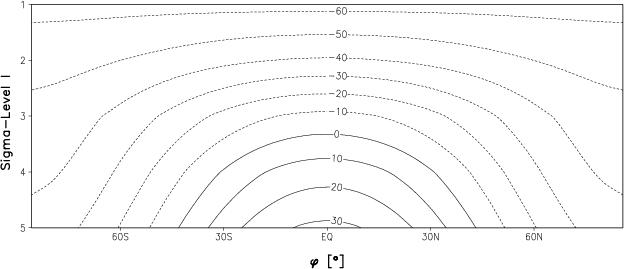
\includegraphics[width=16cm]{Pics/plot_Tr_aqua}
%\centering \epsfig{figure=plot_Tr_aqua.eps, angle=270, width=\linewidth}
\caption{\footnotesize{Restoration temperature field $T_R$ in $\degrees$C as function 
of latitude $\phi$ and the $\sigma$-level $l$ for standard parameter values as in 
figure \ref{Tr_z} and with $(\Delta T_R)_{EP}=70\,K$, $(\Delta T_R)_{NS}=0\,K$.}} \label{Tr_2d}
\end{figure}
}

Usually, for the lower model levels, the time scale $\tau_R$ is set to smaller values 
(stronger diabatic heating) than for the upper levels in order to account for the 
stronger impact of the turbulent heat fluxes near the surface. The standard $\tau_R$ setting 
for $n_l=5$ levels is $(\tau_R)_{l=1,\ldots,3}=30\,d$, $(\tau_R)_{l=4}=10\,d$, 
$(\tau_R)_{l=5}=5\,d$.

\subsection{Diffusion}
\label{diffusion}

The parameterizations (\ref{paraz}), (\ref{parad}) and (\ref{parat}) contain the 
hyperdiffusion terms $H_\zeta$, $H_D$ and $H_T$, respectively. The hyperdiffusion 
parameterizes both the subgrid scale horizontal mixing and the energy cascade into 
these scales and its subsequent dissipation, because the dissipative range of the 
wavenumber-energy-spectrum is not included with the relatively coarse model resolution. 
If $Q$ is one of the model variables $\zeta$, $D$ or $T$, then the hyperdiffusion 
is given by equation (\ref{hypergitter}) for grid point representation and by equation 
(\ref{hyperspektral}) for spectral representation (see also eqn. (\ref{spektral}))
\beqa
H & = & -(-1)^hK\,\nabla^{2h}\,Q(\lambda,\mu,t) \label{hypergitter} \\
  & = & -(-1)^hK\,\nabla^{2h}\sum_\gamma Q_\gamma(t)\,Y_\gamma(\lambda,\mu). \label{hyperspektral}
\eeqa
The hyperdiffusion for one spectral mode $\gamma$ is then \citep{holton}:
\beqa
H_\gamma & = & -(-1)^hK\,\nabla^{2h}\,Q_\gamma(t)\,Y_\gamma(\lambda,\mu) \\
         & = & -K\left(\frac{n(n+1)}{a^2}\right)^hQ_\gamma(t)\,Y_\gamma(\lambda,\mu). \label{hgamma.2}
\eeqa
With the condition that the spectral modes with $n=n_T$ are damped with a prescribed 
time scale $\tau_H$:
\begin{equation}
H_\gamma = -\frac{1}{\tau_H}\,Q_\gamma(t)\,Y_\gamma(\lambda,\mu)\quad\mbox{}
\end{equation}
${if} n=n_T,$ substitution into Equation (\ref{hgamma.2}) yields:
\begin{equation}
K = \frac{1}{\tau_H}\left(\frac{a^2}{n_T(n_T+1)}\right)^h.
\end{equation}
Thus, from Equation (\ref{hgamma.2}) it follows that:
\begin{equation}
H_\gamma = -\frac{1}{\tau_H}\left(\frac{n(n+1)}{n_T(n_T+1)}\right)^hQ_\gamma(t)\,Y_\gamma(\lambda,\mu). \label{hn2}
\end{equation}
In the model the hyperdiffusion is applied in the form (\ref{hn2}). For the shortest 
waves ($n=n_T$) the damping is maximal, for the mean ($n=0$) the damping vanishes. 
The integer exponent with the standard value $h=4$ leads to an additional reduction 
of the damping at small wavenumbers. The diffusion time scale is usually set to
 $\tau_H=1/4\,d$.


\section{Scaling of Variables}
    The variables are rendered dimensionless using the following
     characteristic scales:

\begin{tabular}{|l|l|l|} \hline

Variable    & Scale  & Scale description          \\ \hline \hline
Divergence  & $\Omega$ & $\Omega$  = angular velocity \\ \hline
Vorticity   & $\Omega$ & $\Omega$  = angular velocity \\ \hline
Temperature & $(a^2 {\Omega}^2)/R$ & a = planet radius, R = gas constant \\ \hline
Pressure    & 101100 Pa & PSURF = mean sea level pressure \\ \hline
Orography   & $(a^2 {\Omega}^2)/g$ & g = gravity \\ \hline
\end{tabular}

\section{Vertical Discretization}

\begin{figure}[h]
\setlength{\unitlength}{1cm}
\begin{picture}(14,10)
\thicklines
\multiput(2 ,2)(0,1.5){5}{\line(1,0){8}}
\multiput(10.5,1.25)(0,1.5){5}{\makebox(2,1.5){$\zeta,D,T'$}}
\multiput(10.5,2.00)(0,1.5){4}{\makebox(2,1.5){$\dot{\sigma}$}}
\put(10.5,0.50){\makebox(2,1.5){$p = p_s , \dot{\sigma} = 0$}}
\put(10.5,8.00){\makebox(2,1.5){$p = 0 , \dot{\sigma} = 0$}}
\put(0,8.75){\makebox(1,1.5){$ Level $}}
\put(1,8.75){\makebox(1,1.5){$ \sigma $}}
\put(10.5,8.75){\makebox(2,1.5){$ Variables $}}
\thinlines
\multiput(2,1.25)(0,1.5){6}{\line(1,0){8}}
\put(1,0.50){\makebox(1,1.5){1.0}}
\put(1,1.25){\makebox(1,1.5){0.9}}
\put(1,2.00){\makebox(1,1.5){0.8}}
\put(1,2.75){\makebox(1,1.5){0.7}}
\put(1,3.50){\makebox(1,1.5){0.6}}
\put(1,4.25){\makebox(1,1.5){0.5}}
\put(1,5.00){\makebox(1,1.5){0.4}}
\put(1,5.75){\makebox(1,1.5){0.3}}
\put(1,6.50){\makebox(1,1.5){0.2}}
\put(1,7.25){\makebox(1,1.5){0.1}}
\put(1,8.00){\makebox(1,1.5){0.0}}

\put(0,0.50){\makebox(1,1.5){5.5}}
\put(0,1.25){\makebox(1,1.5){5  }}
\put(0,2.00){\makebox(1,1.5){4.5}}
\put(0,2.75){\makebox(1,1.5){4  }}
\put(0,3.50){\makebox(1,1.5){3.5}}
\put(0,4.25){\makebox(1,1.5){3  }}
\put(0,5.00){\makebox(1,1.5){2.5}}
\put(0,5.75){\makebox(1,1.5){2  }}
\put(0,6.50){\makebox(1,1.5){1.5}}
\put(0,7.25){\makebox(1,1.5){1  }}
\put(0,8.00){\makebox(1,1.5){0.5}}
\end{picture}
\caption{Vertical geometry of PUMA with associated variables (5 level version)}
\label{figlevel}
\end{figure}
    
The model is represented by finite differences in the vertical
as shown in figure \ref{figlevel}. The number of vertical levels 
is variable. The vertical coordinate is defined as $\sigma  = p/p_s$.
The prognostic variables $\zeta,D$, and $T'$ are calculated at full levels.
At the two outer half levels $\sigma = 0$ (upper boundary) and 
$\sigma = 1$ (lower boundary) the vertical velocity is set to zero. 
The vertical advection at level $r$ is approximated as follows:

\begin{equation}
\left( \overline{\dot{\sigma} \delta_{\sigma} Q_{\sigma}} \right)_r = 
\frac{1}{2} \left(
\dot{\sigma}_{r+\frac{1}{2}}
\frac{Q_{r+1}-Q_r}{\Delta \sigma}
+ \dot{\sigma}_{r-\frac{1}{2}}
\frac{Q_r - Q_{r-1}}{\Delta \sigma}
\right)
\end{equation}

The tendencies  of temperature, divergence and surface pressure
are solved by the implicit time step. The vorticity equation
is approximated by the centred differences in time \citep{hossim75}.
    
\section{PUMA Flow Diagram}

\begin{figure}[h]
\setlength{\unitlength}{1cm}
\begin{picture}(14,18)
\thicklines
\newsavebox{\srbox}
\savebox{\srbox}(0,0){
   \thicklines
   \put(0,-0.3){\oval(2.5,0.6)}}
\newsavebox{\cobox}
\savebox{\cobox}(0,0){
   \thinlines
   \put(0,-0.3){\fbox}}
\put(0,16){\usebox{\srbox}\makebox(0,0){puma}}
\put(8,15.9){\fbox{Main program}}
\put(1.25,16){\line(1,0){0.75}}
\put(2,16){\vector(0,-1){0.7}}
\put(2,15){\usebox{\srbox}\makebox(0,0){mpstart}}
\put(8,14.9){\fbox{Multi processing startup}}
\put(2,14.7){\vector(0,-1){0.4}}
\put(2,14){\usebox{\srbox}\makebox(0,0){prolog}}
\put(8,13.9){\fbox{Call initialization routines}}
\put(2,13.7){\vector(0,-1){0.4}}
\put(2,13){\usebox{\srbox}\makebox(0,0){master}}
\put(8,12.9){\fbox{Perform time loop for NRUN time steps}}
\put(3.25,13){\line(1,0){0.75}}
\put(4,13){\vector(0,-1){0.7}}
\put(4,12){\usebox{\srbox}\makebox(0,0){gridpoint}}
\put(8,11.9){\fbox{Call transformation and grid point routines}}
\put(5.25,12){\line(1,0){0.75}}
\put(6,12){\vector(0,-1){0.7}}
\put(6,11){\usebox{\srbox}\makebox(0,0){sp2fc}}
\put(8,10.9){\fbox{Inverse Legendre transformation}}
\put(6,10.7){\vector(0,-1){0.4}}
\put(6,10){\usebox{\srbox}\makebox(0,0){dv2uv}}
\put(8,9.9){\fbox{Divergence and vorticity to u,v - wind components}}
\put(6, 9.7){\vector(0,-1){0.4}}
\put(6, 9){\usebox{\srbox}\makebox(0,0){fc2gp}}
\put(8,8.9){\fbox{Fourier coefficients to grid points (Inverse FFT)}}
\put(6, 8.7){\vector(0,-1){0.4}}
\put(6, 8){\usebox{\srbox}\makebox(0,0){\bf calcgp}}
\put(8,7.9){\fbox{Calculations in grid point space}}
\put(6, 7.7){\vector(0,-1){0.4}}
\put(6, 7){\usebox{\srbox}\makebox(0,0){gp2fc}}
\put(8,6.9){\fbox{Grid point to Fourier coefficients (FFT)}}
\put(6, 6.7){\vector(0,-1){0.4}}
\put(6, 6){\usebox{\srbox}\makebox(0,0){mktend}}
\put(8,5.9){\fbox{Make tendencies for spectral domain}}
\put(6, 5.7){\vector(0,-1){0.4}}
\put(6, 5){\usebox{\srbox}\makebox(0,0){mpsumsc}}
\put(8,4.9){\fbox{MP sum and scatter}}
\put(4, 5){\line(1,0){0.75}}
\put(4, 5){\vector(0,-1){0.7}}
\put(4, 4){\usebox{\srbox}\makebox(0,0){outsp}}
\put(8,3.9){\fbox{Write prognostic fields to file (puma\_data)}}
\put(4, 3.7){\vector(0,-1){0.4}}
\put(4, 3){\usebox{\srbox}\makebox(0,0){diag}}
\put(8,2.9){\fbox{Write diagnostics to standard output}}
\put(4, 2.7){\vector(0,-1){0.4}}
\put(4, 2){\usebox{\srbox}\makebox(0,0){\bf spectral}}
\put(8,1.9){\fbox{Perform spectral calculations and time stepping}}
\put(2, 2){\line(1,0){0.75}}
\put(2, 2){\line(0,1){10}}
\put(2,  7){\makebox(0,0){time \hspace{2mm} loop}}
\put(2, 12){\vector(1,0){0.75}}
\put(4, 1.7){\line(0,-1){0.7}}
\put(4, 1){\vector(-1,0){0.75}}
\put(2, 1){\usebox{\srbox}\makebox(0,0){epilog}}
\put(8,0.9){\fbox{Write restart file (puma\_status)}}
\put(2, 0.7){\vector(0,-1){0.4}}
\put(2, 0){\usebox{\srbox}\makebox(0,0){mpstop}}
\put(8,-0.1){\fbox{MP terminate (end all processes)}}
\end{picture}
\caption{Flow diagram of main routines}
\label{figflow}
\end{figure}


The diagram \ref{figflow} shows the route through the main program
PUMA, with the names of the most important subroutines.
    
    PUMA is the main program. It calls the three subroutines {\sub Prolog},
    {\sub Master}  and {\sub Epilog} .
    {\sub Prolog}  does all initialization. It calls the following subroutines:
    {\sub gauaw} computes gaussian abscissas and weights.
    {\sub inilat} initializes some utility arrays like square of cosine of latitude etc.
    {\sub legpri} prints the arrays of {\sub gauaw} and {\sub inilat}.
    {\sub readnl} reads the namelist from standard input.
    {\sub initpm} initializes most vertical arrays and some in the spectral domain.
    {\sub initsi} computes arrays for the semi-implicit scheme.
    {\sub legini} computes all polynomials needed for the Legendre transformation.
    {\sub restart} starts the model from the restart file, if selected of a previous run.
    {\sub initfd} initializes spectral arrays.
    {\sub setzt} sets up the restoration temperature array.
    {\sub noise} puts a selectable form of noise into $lnPs$.
    {\sub setztex} is a special version of setzt for dipole experiments.
    
    {\sub Master} does some initial timesteps on initial runs, then it runs the 
    time loop for the  selected integration time. It calls the following subroutines:
    {\sub makebm} constructs the array bm, {\sub gridpoint} does all transformations 
    and calculations in the grid point domain. {\sub sp2fc} converts spectral to 
    Fourier coefficients (inverse Legendre transf.), {\sub dv2uv} divergence and 
    vorticity to u and v (implies spectral to Fourier), {\sub fc2gp} Fourier 
    coefficients to grid points (fast Fourier transformation), {\sub calcgp} 
    calculations in grid point space, {\sub gp2fc} grid points to Fourier coefficients 
    (fast Fourier transformation), {\sub fc2sp} Fourier coefficients to spectral 
    (direct Legendre transf.), {\sub mktend} makes tendencies (implies Fourier to spectral),
    {\sub spectral} does all calculations in the spectral domain, {\sub outsp} 
    writes spectral fields in physical dimensions on an output file, and
    {\sub diag} writes selected fields and parameters to the standard output.
    {\sub Epilog} writes the restart file.
    
    
\section{Initialization}
    
    The model starts either from a restart file or with the atmosphere
     at rest. The defaults make the initial state a motionless, stable
     stratified atmosphere. For an initial start the divergence and
     the relative vorticity are set to zero (only mode(1,0) of vorticity
     is set to the planetary vorticity). The temperature is initialized
     as a constant horizontal field. The vertical distribution is
     adopted from the restoration temperature, usually a stable stratification.
     The initialization of the logarithm of the surface pressure
     is controlled by the namelist variable \textbf{kick}:
     \textbf{kick}=0 sets all modes to zero, so the model runs with constant 
     zones without eddies, \textbf{kick}=1 generates random white noise and
     \textbf{kick}=2 generates random white noise that is symmetrical about the equator.
     Runs started with \textbf{kick}=1 or 2 are irreproducible due to the randomization.
     For reproducible runs with eddies use \textbf{kick}=3 which only initializes mode(1,2)
     of $lnPs$ with a small constant.
     The amplitude of the noise perturbation is normalized to 0.1 hPa
     (1.e-4 of the mean surface pressure).
    
     A radiative equilibrium temperature field for the run is set
     up by {\sub setzt}: First, a global mean radiative equilibrium
     temperature profile $T_R(\sigma)$ is defined.
     A hyperbolic function of height is used to provide
     $T_R(\sigma)$, as illustrated in Figure \ref{Tr_z}.
     With $z \rightarrow{} - \infty$ the profile tends to a uniform lapse rate,
     \textbf{alr}, passing through the temperature \textbf{tgr} at \textit{z} = 0.
     With $z \rightarrow{} + \infty$ the profile becomes isothermal. The transition
     takes place at the height \textbf{ztrop}. The sharpness of the tropopause
     is controlled by the parameter \textbf{dttrp}.
     When \textbf{dttrp} = 0,the lapse rate changes discontinuously at \textbf{ztrop}.
     For \textbf{dttrp} small but positive, the transition is spread. The hydrostatic
     relation is used to determine the heights and hence the temperatures
     of the model levels. 
    
\section{Computations in spectral domain}
     The subroutine{\sub spectral} performs one timestep. Details of the time 
     stepping scheme are 
     given in \citep{hossim75}. The adiabatic tendencies
     (advection, etc.) are used. The normal time step is centered in
     time, and includes a Robert time filter to control time splitting.
     For the first \textbf{nkits} time steps, short initial time steps, an initial 
     forward timestep
     followed by a centred step, each twice its predecessor, are taken
     in order to initiate a run from data at only one time level.
     No Robert filter is included in the short steps. The subroutine
     calculates the spectral tendencies due to Newtonian cooling, Rayleigh
     friction and hyperdiffusion:
    
\chapter{Preprocessor}
In many cases the setup of PUMA experiments can be defined
using namelist variables either via MoSt or with editing
the namelist file. In these cases PUMA can run without
any startup files containing boundary conditions. \\

For more complex experiments, like changes in orography
or ground temperature, predefined vertical and horizontal
gradients of the restoration temperature field
and more, it is necessary to create files for boundary
conditions. \\

This is done with the PPP (short for Puma Pre-Processor).

The PPP is a stand alone program, that can be called
inside the modelstarter MoSt or explicitely by the user.
It shares the namelist file {\bf puma\_namelist} with
PUMA, because both programs must use the same parameters
for consistency.

The use in MoSt is currently restricted for using an orography
in PUMA. If the orography option is checked in MoSt the 
PPP will be run before creating the run time environment for
the model. The PPP creates startup definitions for 
orography, constant and time variable part of the restoration
temperature and an initial field for surface pressure.

Additionally the simple orography modifier of MoSt may be used
to rise or lower parts of the orography. A mouseclick on the
button {\bf Preprocess} will then call the PPP and make
all necessary adjustions to start fields. \\
More complex setups must be performed by either using some of
the PPP namelist parameters or by adding code to PPP itself.
This requires however a good knowledge of the FORTRAN-90
programming language and of the model interna.
The source code is in the file Most16/puma/src/ppp.f90.
To make changes easier the PPP has two subroutines
named {\bf modify\_orography} and {\bf modify\_ground\_temperature}.
These are the recommended places to add user code. \\

More details can be found in the FORTRAN-90 code of the PPP itself.



\chapter{Benchmark}
\section{Performance}

\begin{figure}
   \centering
   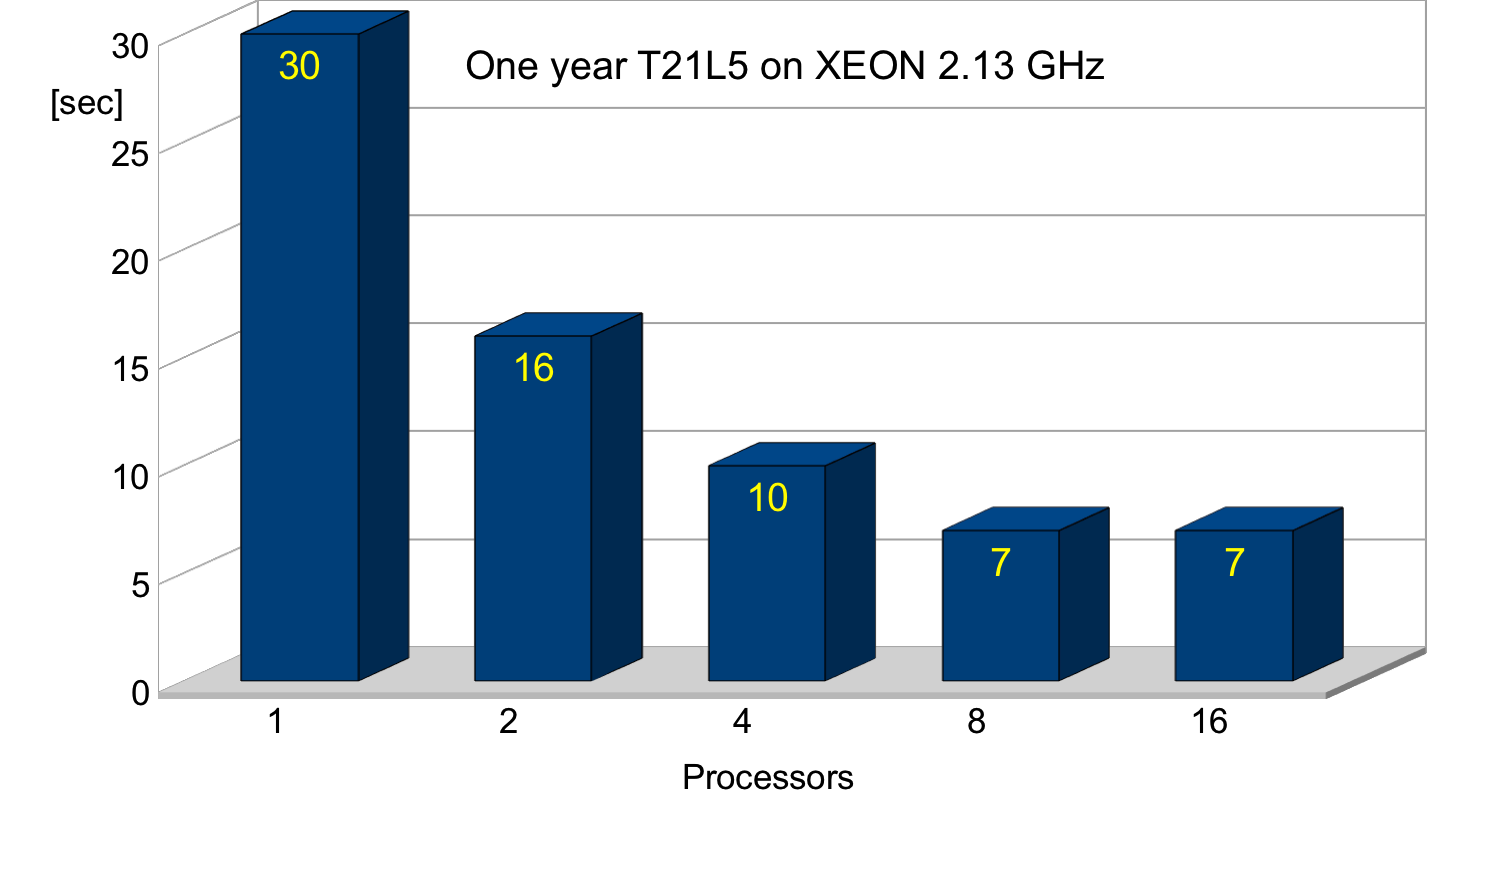
\includegraphics[width=16cm]{Pics/pumat21.png}
   \caption[]{PUMA T21 scaling}
   \label{pumat21}
\end{figure}

{\bf PUMA} on XEON server


\bibliography{ref}
\begin{appendix}
\chapter{List of Constants and Symbols}
\label{locs}
\begin{tabular*}{\textwidth}{|l@{\extracolsep\fill}lll|}
\hline
\vspace{-3mm} & & & \\
Symbol         & Definition                       & Value   & Unit \\
\hline 
\vspace{-3mm} & & & \\
$a$       & earth radius                          & $\rm 6371\e{3}$ & $\rm
m$ \\
$A$       & $=D+\vec{V} \cdot \nabla \ln p_s $         &         & $\rm -$ \\
${\cal A}$      &  absorptivity/emissivity                                           &                     & $\rm -$ \\
${\cal A}_S$  & surface emissivity                                              &         &$\rm -$ \\
$B(T)$            & Planck function                    &    &$\rm Wm^{-2}$ \\
$cc$      & cloud cover                 &    & $\rm -$\\
$C_{char}$     & Charnock constant                     & 0.018   & $\rm -$ \\
$C_h$          & transfer coefficient for heat         &         & $\rm -$ \\
$C_m$          & drag coefficient for momentum         &         & $\rm -$ \\
$c_p$          & specific heat of moist air at constant pressure      &         & $\rm J\,
kg^{-1}\, K^{-1}$ \\  
$c_{pd}$  & specific heat of dry air at constant pressure   & 1005.46      & $\rm J\,
kg^{-1}\, K^{-1}$ \\
$c_{pv}$  & specific heat of water vapor at constant pressure    & 1869.46      & $\rm J\,
kg^{-1}\, K^{-1}$ \\
$c_{p_i}$      & specific heat of sea ice              & 2070         & $\rm W\,
s\, kg^{-1}\, K^{-1}$ \\
$c_{p_s}$      & specific heat of snow            & 2090         & $\rm W\,
s\, kg^{-1}\, K^{-1}$ \\
$c_{p_w}$      & specific heat of sea water            & 4180         & $\rm W\,
s\, kg^{-1}\, K^{-1}$ \\
$c_w$          & coefficient for the deep ocean heat flux   & 4       & $\rm W\,
m^{-2}\, K^{-1}$ \\
$C_w$          & wetness factor                   &         & $\rm -$ \\

$D$       & scaled divergence                          &         & $\rm -$ \\

$E$       & evaporation                      &         & $\rm m\,
s^{-1}$ \\
$E_0$          & extrateristical solar flux density         &         & $\rm W\,
m^{-2}$ \\

$f$       & Coriolis parameter $=:2\Omega\sin\varphi$  &         & $\rm
s^{-1}$ \\
$F_p$          & tendency of the first moment$=:\frac{d R_{1}}{d t}$  &    &
$\rm K\, m^2\, s^{-1}$ \\
$F_q$          & tendency of the zeroth moment$=:\frac{d R_{0}}{d t}$ &    &
$\rm K\, m\, s^{-1}$ \\
$F_q$          & surface moisture flux            &         & $\rm kg\,
m^{-2}\, s^{-1}$ \\
$F_T$          & surface sensible heat flux            &         & $\rm W\,
m^{-2}$ \\
$F_u$          & surface zonal wind stress             &         & $\rm Pa$
\\
$F_v$          & surface meridional wind stress        &         & $\rm Pa$
\\
$F^{LW}$  & long wave radiation flux density      &    &$\rm  W m^{-2}$ \\
$F^{SW}$  & short wave radiation flux density     &    &$\rm  W m^{-2}$ \\
$g$       & gravitational acceleration            & 9.81         & $\rm
m^{-2}$ \\

$h_{mix}$      & mixed layer depth                     &         & $\rm m$ \\
$h_{mix_c}$    & climatological mixed layer depth           &         & $\rm m$ \\
$H_q$          & effective mixed layer depth $=:\frac{R_{0}}{T_{mix}-T_{ref}}$ &
& $\rm m$ \\
$H_p$          & reduced center of gravity $=:\frac{R_{1}}{R_0}$ &         &
$\rm m$ \\ 

\hline
\end{tabular*}
\newpage

\begin{tabular*}{\textwidth}{|l@{\extracolsep\fill}lll|}
\hline
\vspace{-3mm} & & & \\
Symbol         & Definition                       & Value   & Unit \\
\hline 
\vspace{-3mm} & & & \\

$J_q$          & vertical turbulent moisture flux           &         & $\rm kg\, m^{-2}\,
s^{-1}$ \\
$J_T$          & vertical turbulent temperature flux        &         & $\rm K\,
m^{-2}\, s^{-1}$ \\
$J_u$          & vertical turbulent flux of zonal momentum  &         & $\rm Pa$
\\
$J_v$          & vertical turbulent flux of meridional momentum &          & $\rm Pa$
\\

$k$       & von Karman constant                   & 0.4          & $\rm -$ \\
$K_h$          & exchange coefficient for heat         &         & $\rm -$ \\
$K_m$          & exchange coefficient for momentum          &         &$\rm -$ \\
$L$       & latent heat                      &         & $\rm J\, kg^{-1}$\\

$L_f$          & latent heat of fusion = $L_s - L_v$        & $\rm 3.28\e{5}$   &
$\rm J\, kg^{-1}$ \\
$l_h$          & mixing length for heat                &         & $\rm m$ \\
$l_m$          & mixing length for momentum            &         &
$\rm m$ \\
$L_s$          & latent heat of sublimation            & $\rm 2.8345\e{6}$ & $\rm J\,
kg^{-1}$ \\
$L_v$          & latent heat of vapourization               & $\rm 2.5008\e{6}$
     & $\rm J\, kg^{-1}$ \\
$P_c$     & convective precipitation    &    &$\rm  m s^{-1}$ \\
$P_l$     & large scale precipitation   &    &$\rm  m s^{-1}$ \\
$P^m_n(\mu)$   & associated Legendre function of the first kind &          & $\rm -$ \\
$p$       & pressure  \hspace*{\fill}             &         & $\rm Pa$ \\
$p_S$          & surface pressure                 &         & $\rm Pa$
\\
$p_s$          & scaled surface pressure               &         & $\rm -$ \\

$q$       & specific humidity                     &         & $\rm kg\,
kg^{-1}$ \\
$Q$       & total heat flux through sea ice       &         & $\rm W\, m^{-2}$
\\
$\tilde{Q}$    & flux correction heat flux through sea ice  &         & $\rm W\, m^{-2}$
\\
$Q_a$          & total atmospheric heat flux                &         & $\rm W\,
m^{-2}$ \\
$Q_c$          & conductive heat flux through sea ice       &         & $\rm W\,
m^{-2}$ \\
$Q_f$          & heat flux available for freezing sea ice   &         & $\rm W\, m^{-2}$
\\
$Q_g$     & heat flux into the soil     &    & $\rm W m^{-2}$ \\
$Q_m$     & snow melt heat flux    &    & $\rm W m^{-2}$ \\
$Q_o$          & oceanic heat flux                     &         & $\rm W\, m^{-2}$
\\
$q_S$          & surface specific humidity             &         & $\rm kg\,
kg^{-1}$ \\
$q_{sat}$      & saturation specific humidity               &         & $\rm kg\,
kg^{-1}$ \\
${\cal R}$     & refexivity/albedo      &    &$\rm -$ \\
${\cal R}_S$   & surface albedo    &    & $\rm -$ \\
$R_d$          & gas constant for dry air              & 287.05  & $\rm J\,
kg^{-1}\, K^{-1}$ \\
$R_l$          & surface long wave radiation           &         & $\rm W\,
m^{-2}$ \\
$R_s$          & surface short wave radiation               &         & $\rm W\,
m^{-2}$ \\
$R_v$          & gas constant for water vapor               & 461.51  &
$\rm J\, kg^{-1}\, K^{-1}$ \\
$R_{0}$   & zeroth moment of the temperature distribution   &         & $\rm K\,
m$ \\
$R_{1}$   & first moment of the temperature distribution    &         & $\rm K\,
m^2$ \\
$Ri$           & Richardson number                     &         & $\rm -$ \\ 
$S_w$          & salinity of sea water                 & 34.7    
     & $\rm psu$ \\

\hline
\end{tabular*}
\newpage

\begin{tabular*}{\textwidth}{|l@{\extracolsep\fill}lll|}
\hline
\vspace{-3mm} & & & \\
Symbol         & Definition                       & Value   & Unit \\
\hline 
\vspace{-3mm} & & & \\

$t$       & time                             &         & $\rm s$ \\
$t$       & scaled time step                      &         & $\rm -$ \\
${\cal T}$     & transmissivity    &    &$\rm  -$ \\
$T$       & temperature                      &         & $\rm K$
\\
$T'$           & temperature anomaly $=:T-T_0$              &         & $\rm -$ \\
$T_d$          & deep ocean temperature (at 400m)      &         & $\rm K$
\\
$T_i$          & sea ice surface temperature           &         & $\rm K$ \\
$T_f$          & freezing temperature                  & 271.25  & $\rm K$
\\
$T_s$          & surface temperature                   &         & $\rm K$
\\
$T_{sea}$ & sea surface temperature     &    & $\rm K$ \\
$T_{melt}$     & melting point                    & 273.16  & $\rm K$ \\
$T_{mix}$      & mixed layer temperature               &         & $\rm K$ \\
$T_{mix_c}$    & climatological mixed layer temperature     &         & $\rm K$
\\
$T_{ref}$      & asymptotic reference temperature           &         & $\rm K$ \\
$T_w$          & oceanic temperature profile                &         &
$\rm K$ \\
$T_0$          & reference temperature profile         &  250.0  & $\rm K$
\\

$U$       & scaled zonal wind $=:u\cdot\cos\varphi$    &         & $\rm -$ \\
$u$       & zonal wind                       &         & $\rm m\, s^{-1}$
\\
$u_*$          & friction velocity                          &         & $\rm m\, s^{-1}$ \\

$V$       & scaled meridional wind $=:v\cdot\cos\varphi$    &         & $\rm -$ \\
$v$       & meridional wind                  &         & $\rm m\, s^{-1}$
\\
$\vec{v}$      & horizontal wind vector                &         & $\rm m\, s^{-1}$
\\
$W_L$     & cloud liquid water path     &    & $\rm g m^2$ \\
$W_{snow}$ & mass of snow water    &    & $\rm kg $\\
$W_{soil}$     & soil water             &    & $\rm  m $\\
$z$       & height                      &    & $\rm m$ \\
$z_0$          & roughness length            &    & $\rm m$ \\
$\Delta t $    & time increment              &    & $\rm s$ \\
 $\Delta z $   & height increment            &    &$\rm  m$ \\
$\alpha$  & thermal expansion coefficient $\frac{1}{\rho} \frac{d\rho}{dT}$ & $\rm
2.41\e{-4}$ & $\rm K^{-1}$ \\
$\beta$   & back scattering coefficient &         &$\rm - $\\
$\beta_d$      & diffusivity factor          & 1.66    &$\rm - $ \\
$\zeta$   & scaled vorticity                      &         & $\rm -$ \\
$\theta$  & potential temperature            &         & $\rm K$ \\
$\kappa$  & $R_d/C_{pd}$                               &         & $\rm -$ \\
$\bar{\kappa}$      & mean heat conductivity in ice and snow     &         & $\rm W\,
m^{-1}\, K^{-1}$ \\
$\kappa_i$     & heat conductivity in ice              &  2.03   & $\rm W\, m^{-1}\,
K^{-1}$ \\
$\kappa_s$     & heat conductivity in snow             &  0.31   & $\rm W\,
m^{-1}\, K^{-1}$ \\

$\lambda_h$    & asymptotic mixing length for heat     &    &$\rm m $\\
$\lambda_m$    & asymptotic mixing length for momentum      &    &$\rm m $\\

$\lambda$      & longitude                                  &         & $\rm -$ \\

$\mu$          & $\sin\varphi$                              &         & $\rm -$ \\
$\mu_0$   & cosine of the solar zenith angle           &         & $\rm -$ \\ 

$\rho$         & density of air                   &         & $\rm kg\,
m^{-3}$ \\
$\rho_i$  & density of sea ice                    & 920          & $\rm kg\, m^{-3}$
\\
$\rho_s$  & density of snow                       & 330          & $\rm kg\, m^{-3}$
\\
$\rho_w$  & density of sea water                  & 1030         & $\rm kg\,
m^{-3}$ \\
$\rho_o$  & density of fresh water                & 1000    & $\rm kg\, m^{-3}$
\\

\hline
\end{tabular*}
\newpage

\begin{tabular*}{\textwidth}{|l@{\extracolsep\fill}lll|}
\hline
\vspace{-3mm} & & & \\
Symbol         & Definition                       & Value   & Unit \\
\hline 
\vspace{-3mm} & & & \\
$\sigma$  & normalized pressure coordinate $=: p/p_s$       &         & $\rm -$ \\
$\dot{\sigma}$  & vertical velocity in $\sigma$ system           &         & $\rm -$ \\
$\sigma_{SB}$ & Stefan-Bolzmann constant & $ 5.67 \e{-8}$ &$\rm W m^{-2}K^{-4}$ \\
$\tau_N$  & cloud optical depth    &    &$\rm  -$\\
$\tau_{F}$     & time scale for RF                     &         & $\rm -$ \\
$\tau_{R}$     & time scale for NC                     &         & $\rm -$ \\
$\tau_{T}$     & time scale for temperature flux correction      &         & $\rm s$ \\
$\tau_{h}$     & time scale for depth flux correction            &         & $\rm s$ \\

$\phi$         & geopotential height $:=g\cdot{z}$          &         & $\rm m^2\,
s^{-2}$ \\
$\phi$         & scaled geopotential height            &         & $\rm -$ \\
$\varphi$      & latitude                                   &         & $\rm -$ \\

$\chi$    & scaled velocity potential                  &         & $\rm -$ \\

$\psi$         & scaled streamfunction                      &         & $\rm -$ \\
$\Omega$  & angular velocity of the earth              & $\rm 7.292\e{-5}$ & $\rm
s^{-1}$ \\
$\tilde{\omega_0}$ & single scattering albedo     &    &$\rm- $\\

\hline
\end{tabular*}


\chapter{PUMA Codes for Variables}
\label{Pumacodes}
\documentclass[a4paper,12pt]{article}
\parindent0.0em
\parskip1.5ex plus 0.5ex minus 0.5ex
\begin{document}

\begin{table}[t]
Codes available from PUMA-burner (adapted from ECHAM) \\

\begin{tabular}[t]{|l|l|l|l|l|} \hline
\multicolumn{1}{|c|}{Code} &
\multicolumn{1}{c|}{Levels}&
\multicolumn{1}{c|}{Type} &
\multicolumn{1}{c|}{Variable} &
\multicolumn{1}{c|}{Unit} \\ \hline \hline

110 & 1    & g  & mixed layer depth                & m               \\ \hline
129 & 1    & s  & surface geopotential             & m$^{2}$/s$^{2}$ \\ \hline
130 & NLEV & s  & temperature                      & K               \\ \hline
131 & NLEV & c  & u-velocity                       & m/s             \\ \hline
132 & NLEV & c  & v-velocity                       & m/s             \\ \hline
133 & NLEV & s  & specific humidity                & kg/kg           \\ \hline
135 & NLEV & c  & vertical velocity                & Pa/s            \\ \hline
138 & NLEV & s  & vorticity                        & 1/s             \\ \hline
139 & 1    & g  & surface temperature              & K               \\ \hline
140 & 1    & g  & soil wetness                     & m               \\ \hline
141 & 1    & g  & snow depth (water equi.)         & m               \\ \hline
142 & 1    & ga & large scale precipitation        & m/s             \\ \hline
143 & 1    & ga & convective precipitation         & m/s             \\ \hline
144 & 1    & ga & snow fall                        & m/s             \\ \hline
146 & 1    & ga & surface sensible heat flux       & W/m$^{2}$       \\ \hline
147 & 1    & ga & surface latent heat flux         & W/m$^{2}$       \\ \hline
148 & NLEV & c  & horizontal streamfunktion        & m$^{2}$/s       \\ \hline
149 & NLEV & c  & velocity potential               & m$^{2}$/s       \\ \hline
151 & 1    & c  & mean sea level pressure          & Pa              \\ \hline
152 & 1    & s  & ln(surface pressure)             &                 \\ \hline
153 & NLEV & g  & cloud liquid water content       & kg/kg           \\ \hline
155 & NLEV & s  & divergence                       & 1/s             \\ \hline
156 & NLEV & c  & geopotential height              & gpm             \\ \hline
157 & NLEV & c  & relative humidity                & frac.           \\ \hline
159 & 1    & g  & (u$^{\star}$)$^{3}$              & (m/s)$^{3}$     \\ \hline
160 & 1    & ga & surface runoff                   & m/s             \\ \hline

\end{tabular}

\end{table}

\begin{table}[t]

\begin{tabular}[t]{|l|l|l|l|l|} \hline
\multicolumn{1}{|c|}{Code} &
\multicolumn{1}{c|}{Levels}&
\multicolumn{1}{c|}{Type} &
\multicolumn{1}{c|}{Variable} &
\multicolumn{1}{c|}{Unit} \\ \hline \hline

162 & NLEV & g  & cloud cover                      & frac.           \\ \hline
164 & 1    & ga & total cloud cover                & frac.           \\ \hline
169 & 1    & ga & surface temperature              & K               \\ \hline
170 & 1    & g  & deep soil temperature            & K               \\ \hline
172 & 1    & g  & land sea mask                    & [0:sea,1:land]   \\ \hline
173 & 1    & g  & surface roughness                & m               \\ \hline
175 & 1    & g  & surface albedo                   & frac.           \\ \hline
176 & 1    & ga & surface solar radiation          & W/m$^{2}$       \\ \hline
177 & 1    & ga & surface thermal radiation        & W/m$^{2}$       \\ \hline
178 & 1    & ga & top solar radiation              & W/m$^{2}$       \\ \hline
179 & 1    & ga & top thermal radiation            & W/m$^{2}$       \\ \hline
180 & 1    & ga & u-stress                         & Pa              \\ \hline
181 & 1    & ga & v-stress                         & Pa              \\ \hline
182 & 1    & ga & evaporation                      & m/s             \\ \hline
183 & 1    & g  & soil temperature                 & K               \\ \hline
203 & 1    & ga & top solar radiation upward       & W/m$^{2}$       \\ \hline
204 & 1    & ga & surface solar radiation upward   & W/m$^{2}$       \\ \hline
205 & 1    & ga & surface thermal radiation upward & W/m$^{2}$       \\ \hline
207 & 1    & g  & soil temperature (level 2)       & K               \\ \hline
208 & 1    & g  & soil temperature (level 3)       & K               \\ \hline
209 & 1    & g  & soil temperature (level 4)       & K               \\ \hline
210 & 1    & g  & sea ice cover                    & frac.           \\ \hline
211 & 1    & g  & sea ice thickness                & m               \\ \hline
212 & 1    & g  & vegetation cover                 & frac.           \\ \hline
218 & 1    & g  & snow melt (water equiv.)         & m/s             \\ \hline
221 & 1    & g  & snow depth change (water equiv.) & m/s             \\ \hline
230 & 1    & ga & vertical integrated spec. hum.   & kg/m$^{2}$      \\ \hline
232 & 1    & g  & glacier cover                    & frac.           \\ \hline

\end{tabular}

\vspace*{0.5cm}

s: PUMA spectral field; g: PUMA grid point field; c: computed by PUMA-burner;
a: accumulated

\end{table}


\end{document}


\chapter{Namelist}
\label{Namelist}
\begin{tabular}{|l|r|l|}                                  
\hline                                                        
Name   & Default & Description \\
\hline
& & \\
{\bf nlat    } &  32 & 0: Number of latitudes \\
{\bf nlev    } &  10 & 1: Number of levels    \\
& & \\
\hline                                                        
\end{tabular}



\newpage
\begin{tabular}{|l|r|l|}                                  
\hline                                                        
Name   & Default & Description \\
\hline
& & \\
{\bf kick    } &  1 & 0: no initial noise ($p_s$ = const.) \\
{\bf         } &    & 1: initial random white noise        \\
{\bf         } &    & 2: equator symmetric random white noise   \\
{\bf         } &    & 3: mode (1,2) reproducable initialization \\
{\bf lat1oro } &    & used in preprocessor \\
{\bf lat1tgt } &    & used in preprocessor \\
{\bf lat2oro } &    & used in preprocessor \\
{\bf lat2tgr } &    & used in preprocessor \\
{\bf lon1oro } &    & used in preprocessor \\
{\bf lon1tgt } &    & used in preprocessor \\
{\bf lon2oro } &    & used in preprocessor \\
{\bf lon2tgr } &    & used in preprocessor \\
{\bf nafter  } & 24 & outputinterval: obsolete, replaced by nwpd \\
{\bf ncoeff  } &  0 & number of coefficients to print in {\bf wrspam} \\  
{\bf ncorrect} &    & used in preprocessor \\
{\bf ncu     } &  0 & $ncu > 0$ : write debug info to file unit (ncu) \\
{\bf ndel    } &  6 & order of hyperdiffusion for each level (2*h) \\
{\bf ndiag   } & 12 & output interval for diagnostics [timesteps] \\   
{\bf nextout } &  0 & extended output: ps at t-1 and t-2 \\
{\bf nfls    } &    & used in preprocessor \\
{\bf ngui    } &  0 & 1: run with GUI \\
{\bf nguidbg } &  0 & 1: switch on GUI debug output \\
{\bf nhz     } &  0 & $nhz > 0$: Held \& Suarez setups \\
{\bf nkits   } &  3 & number of short initial timesteps \\       
{\bf nlevt   } &  0 & number of tropospheric levels (if nvg = 1) \\
{\bf nextout } &  0 & 1:extended output (entropy production) \\
{\bf nmonths } &  0 & simulation time in months \\
{\bf noro    } &    & used in preprocessor \\
{\bf norox   } &    & used in preprocessor \\
{\bf noutput } &  1 & 1:write model output to file {\bf puma\_output} \\
{\bf nreverse} &    & used in preprocessor \\
{\bf nruido  } &  0 & 1:add noise on every time step \\
{\bf nrun    } &  0 & number of timesteps to run - 0: use nyears and nmonths \\
{\bf nsponge } &  0 & 1:use sponge layer at top \\
{\bf nsrv    } &    & used in preprocessor \\
{\bf nstep   } &  0 & current timestep \\
{\bf nstop   } &  0 & stop step - 0: compute from nyears 6 nmonths \\
{\bf nstrato } &    & used in preprocessor \\
{\bf ntgr    } &    & used in preprocessor \\
{\bf ntspd   } & 24 & number of time steps per day  \\         
{\bf nvg     } &  0 & vertical grid type 0:linear 1:Scinocca 2:Polvani \\
{\bf nwpd    } &  1 & number of writes per day (to {\bf puma\_output}) \\
{\bf nwspini } &  1 & 1: Write initial sp(:) to file {\bf puma\_sp\_ini}\\
{\bf nyears  } &  1 & simulation time in years  \\
{\bf nyoden  } &    & used in preprocessor \\
& & \\
\hline                                                        
\end{tabular}
\newpage

\begin{tabular}{|l|r||l|}                                  
\hline
Name   & Default & Description \\
\hline
& & \\
{\bf alrpv  } &      & used in preprocessor \\
{\bf alrs   } &      & used in preprocessor \\
{\bf disp   } &  0.0 & noise amplitude for nruido = 1 \\
{\bf dorox  } &      & used in preprocessor \\
{\bf doroxs } &      & used in preprocessor \\
{\bf doroy  } &      & used in preprocessor \\
{\bf doroys } &      & used in preprocessor \\
{\bf dt     } &      & used in preprocessor \\
{\bf dtep   } & 60.0 & temperature difference at surface for $T_R$ \\
{\bf        } &      & equator - pole (forcing) \\
{\bf dtns   } &  0.0 & temperature difference at surface for $T_R$  \\ 
{\bf        } &      & North pole - South pole (season simulation) \\
{\bf dtrop  } & 12000.0 & height of tropopause [m] \\ 
{\bf dttrp  } &  2.0 & temperature increment controlling the sharpness \\ 
{\bf        } &      & of the tropopause in $T_R$ \\
{\bf dtzz   } &      & used in preprocessor \\
{\bf dvdiff } & 0.0  & vertical diffusion coefficient \\
{\bf edgepv } &      & used in preprocessor \\
{\bf flsamp } &      & used in preprocessor \\
{\bf flsdp  } &      & used in preprocessor \\
{\bf flsp0  } &      & used in preprocessor \\
{\bf flsoff } &      & used in preprocessor \\
{\bf horo   } &      & used in preprocessor \\
{\bf oroano } &      & used in preprocessor \\
{\bf orofac } &      & used in preprocessor \\
{\bf pac    } &  0.0 & phase  of annual cycle in [days] \\
{\bf pmaxpv } &      & used in preprocessor \\
{\bf pspon  } & 50.0 & sponge layer limit \\
{\bf psurf  } & 101100.0 & global mean sea level pressure [Pa] \\
{\bf radpv  } &      & used in preprocessor \\
{\bf rotspd } &  1.0 & Earth rotation speed factor \\
{\bf sigmax } &  0.0 & sigma value of top half level \\
{\bf sponk  } &  0.5 & max. damping coefficient in sponge layer \\
{\bf tac    } &  0.0 & length of annual cycle in [days] \\
{\bf tauta  } & 40.0 & far surface heating time scale $nhz > 0$ \\
{\bf tauts  } &  0.0 & near surface heating time scale $nhz > 0$ \\
{\bf tdiss  } &  0.2 & diffusion time scale for divergence [days] \\
{\bf tgr    } & 288.0 & global mean temperature of ground used to set $T_R$ \\ 
{\bf tgrano } & 0.0  & used in preprocessor \\
{\bf ttp    } &      & used in preprocessor \\
& & \\
\hline
\end{tabular}

\begin{tabular}{|l|l|r|r||l|}                                  
\hline
Name   & Type & Dimension & Default & Description \\
\hline
& & & & \\
{\bf ndl      } & integer & NLEV & 0 & 1: activate spectral printouts for this level \\
{\bf restim   } & real    & NLEV & 15.0 & restoration timescale for each level \\ 
{\bf sigmah   } & real    & NLEV &  0.0 & define your own half-level layout \\
{\bf t0k      } & real    & NLEV & 250.0 & reference $T_R$-temperature profile \\ 
{\bf tfrc     } & real    & NLEV & 0,0,0,.. ,1 & Rayleigh friction timescale $\tau_F$ in days \\
{\bf nselect  } & integer & NTP1 &  1 & enable (1) or disable (0) zonal waves \\
{\bf nspecsel } & integer & NCSP &  1 & enable (1) or disable (0) modes \\
& & & & \\
\hline                                                        
\end{tabular}

\end{appendix}

\end{document}
